% Options for packages loaded elsewhere
\PassOptionsToPackage{unicode}{hyperref}
\PassOptionsToPackage{hyphens}{url}
%
% \documentclass[
%   openany]{book}
\documentclass[runningheads]{llncs}
\usepackage{amsmath,amssymb}
\usepackage{lmodern}
\usepackage{ifxetex,ifluatex}
\ifnum 0\ifxetex 1\fi\ifluatex 1\fi=0 % if pdftex
  \usepackage[T1]{fontenc}
  \usepackage[utf8]{inputenc}
  \usepackage{textcomp} % provide euro and other symbols
\else % if luatex or xetex
  \usepackage{unicode-math}
  \defaultfontfeatures{Scale=MatchLowercase}
  \defaultfontfeatures[\rmfamily]{Ligatures=TeX,Scale=1}
\fi
% Use upquote if available, for straight quotes in verbatim environments
\IfFileExists{upquote.sty}{\usepackage{upquote}}{}
\IfFileExists{microtype.sty}{% use microtype if available
  \usepackage[]{microtype}
  \UseMicrotypeSet[protrusion]{basicmath} % disable protrusion for tt fonts
}{}
\makeatletter
\@ifundefined{KOMAClassName}{% if non-KOMA class
  \IfFileExists{parskip.sty}{%
    \usepackage{parskip}
  }{% else
    \setlength{\parindent}{0pt}
    \setlength{\parskip}{6pt plus 2pt minus 1pt}}
}{% if KOMA class
  \KOMAoptions{parskip=half}}
\makeatother
\usepackage{xcolor}
\IfFileExists{xurl.sty}{\usepackage{xurl}}{} % add URL line breaks if available
\IfFileExists{bookmark.sty}{\usepackage{bookmark}}{\usepackage{hyperref}}
\hypersetup{
  pdftitle={Supplementary Materials - CellDepot: A unified repository for scRNAseq data and visual exploration},
  hidelinks,
  pdfcreator={LaTeX via pandoc}}
\urlstyle{same} % disable monospaced font for URLs
\usepackage[margin=2cm]{geometry}
\usepackage{color}
\usepackage{fancyvrb}
\newcommand{\VerbBar}{|}
\newcommand{\VERB}{\Verb[commandchars=\\\{\}]}
\DefineVerbatimEnvironment{Highlighting}{Verbatim}{commandchars=\\\{\}}
% Add ',fontsize=\small' for more characters per line
\usepackage{framed}
\definecolor{shadecolor}{RGB}{248,248,248}
\newenvironment{Shaded}{\begin{snugshade}}{\end{snugshade}}
\newcommand{\AlertTok}[1]{\textcolor[rgb]{0.94,0.16,0.16}{#1}}
\newcommand{\AnnotationTok}[1]{\textcolor[rgb]{0.56,0.35,0.01}{\textbf{\textit{#1}}}}
\newcommand{\AttributeTok}[1]{\textcolor[rgb]{0.77,0.63,0.00}{#1}}
\newcommand{\BaseNTok}[1]{\textcolor[rgb]{0.00,0.00,0.81}{#1}}
\newcommand{\BuiltInTok}[1]{#1}
\newcommand{\CharTok}[1]{\textcolor[rgb]{0.31,0.60,0.02}{#1}}
\newcommand{\CommentTok}[1]{\textcolor[rgb]{0.56,0.35,0.01}{\textit{#1}}}
\newcommand{\CommentVarTok}[1]{\textcolor[rgb]{0.56,0.35,0.01}{\textbf{\textit{#1}}}}
\newcommand{\ConstantTok}[1]{\textcolor[rgb]{0.00,0.00,0.00}{#1}}
\newcommand{\ControlFlowTok}[1]{\textcolor[rgb]{0.13,0.29,0.53}{\textbf{#1}}}
\newcommand{\DataTypeTok}[1]{\textcolor[rgb]{0.13,0.29,0.53}{#1}}
\newcommand{\DecValTok}[1]{\textcolor[rgb]{0.00,0.00,0.81}{#1}}
\newcommand{\DocumentationTok}[1]{\textcolor[rgb]{0.56,0.35,0.01}{\textbf{\textit{#1}}}}
\newcommand{\ErrorTok}[1]{\textcolor[rgb]{0.64,0.00,0.00}{\textbf{#1}}}
\newcommand{\ExtensionTok}[1]{#1}
\newcommand{\FloatTok}[1]{\textcolor[rgb]{0.00,0.00,0.81}{#1}}
\newcommand{\FunctionTok}[1]{\textcolor[rgb]{0.00,0.00,0.00}{#1}}
\newcommand{\ImportTok}[1]{#1}
\newcommand{\InformationTok}[1]{\textcolor[rgb]{0.56,0.35,0.01}{\textbf{\textit{#1}}}}
\newcommand{\KeywordTok}[1]{\textcolor[rgb]{0.13,0.29,0.53}{\textbf{#1}}}
\newcommand{\NormalTok}[1]{#1}
\newcommand{\OperatorTok}[1]{\textcolor[rgb]{0.81,0.36,0.00}{\textbf{#1}}}
\newcommand{\OtherTok}[1]{\textcolor[rgb]{0.56,0.35,0.01}{#1}}
\newcommand{\PreprocessorTok}[1]{\textcolor[rgb]{0.56,0.35,0.01}{\textit{#1}}}
\newcommand{\RegionMarkerTok}[1]{#1}
\newcommand{\SpecialCharTok}[1]{\textcolor[rgb]{0.00,0.00,0.00}{#1}}
\newcommand{\SpecialStringTok}[1]{\textcolor[rgb]{0.31,0.60,0.02}{#1}}
\newcommand{\StringTok}[1]{\textcolor[rgb]{0.31,0.60,0.02}{#1}}
\newcommand{\VariableTok}[1]{\textcolor[rgb]{0.00,0.00,0.00}{#1}}
\newcommand{\VerbatimStringTok}[1]{\textcolor[rgb]{0.31,0.60,0.02}{#1}}
\newcommand{\WarningTok}[1]{\textcolor[rgb]{0.56,0.35,0.01}{\textbf{\textit{#1}}}}
\usepackage{longtable,booktabs,array}
\usepackage{calc} % for calculating minipage widths
% Correct order of tables after \paragraph or \subparagraph
\usepackage{etoolbox}
\makeatletter
\patchcmd\longtable{\par}{\if@noskipsec\mbox{}\fi\par}{}{}
\makeatother
% Allow footnotes in longtable head/foot
\IfFileExists{footnotehyper.sty}{\usepackage{footnotehyper}}{\usepackage{footnote}}
\makesavenoteenv{longtable}
\usepackage{graphicx}
\makeatletter
\def\maxwidth{\ifdim\Gin@nat@width>\linewidth\linewidth\else\Gin@nat@width\fi}
\def\maxheight{\ifdim\Gin@nat@height>\textheight\textheight\else\Gin@nat@height\fi}
\makeatother
% Scale images if necessary, so that they will not overflow the page
% margins by default, and it is still possible to overwrite the defaults
% using explicit options in \includegraphics[width, height, ...]{}
\setkeys{Gin}{width=\maxwidth,height=\maxheight,keepaspectratio}
% Set default figure placement to htbp
\makeatletter
\def\fps@figure{htbp}
\makeatother
\setlength{\emergencystretch}{3em} % prevent overfull lines
\providecommand{\tightlist}{%
  \setlength{\itemsep}{0pt}\setlength{\parskip}{0pt}}
\setcounter{secnumdepth}{5}
\usepackage{booktabs}
\usepackage{amsthm}
\makeatletter
\def\thm@space@setup{%
  \thm@preskip=8pt plus 2pt minus 4pt
  \thm@postskip=\thm@preskip
}
\makeatother
\ifluatex
  \usepackage{selnolig}  % disable illegal ligatures
\fi
\usepackage[]{natbib}
\usepackage{bbding}
% \pagestyple{empty}
\bibliographystyle{apalike}


% \title{Supplementary Materials - CellDepot: A unified repository for scRNAseq data and visual exploration}
% % \author{Dongdong Lin}
% % % \thanks{These two authors contributed equally}
% % \author{Yirui Chen}
% % \thanks{These two authors contributed equally}
% \date{2021-12-09}

\usepackage{graphicx}
\renewcommand\UrlFont{\color{blue}\rmfamily}
\begin{document}

\title{Contribution Title\thanks{Supported by organization x.}}
%
%\titlerunning{Abbreviated paper title}
% If the paper title is too long for the running head, you can set
% an abbreviated paper title here
%
\author{First Author\inst{1}\orcidID{0000-1111-2222-3333} \and
Second Author\inst{2,3}\orcidID{1111-2222-3333-4444} \and
Third Author\inst{3}\orcidID{2222--3333-4444-5555}}
%
\authorrunning{F. Author et al.}
% First names are abbreviated in the running head.
% If there are more than two authors, 'et al.' is used.
%
\institute{Princeton University, Princeton NJ 08544, USA \and
Springer Heidelberg, Tiergartenstr. 17, 69121 Heidelberg, Germany
\email{lncs@springer.com}\\
\url{http://www.springer.com/gp/computer-science/lncs} \and
ABC Institute, Rupert-Karls-University Heidelberg, Heidelberg, Germany\\
\email{\{abc,lncs\}@uni-heidelberg.de}}

\maketitle

{
\setcounter{tocdepth}{1}
\tableofcontents
}
\hypertarget{preface}{%
\chapter{Preface}\label{preface}}

This is a **supplementary materials* written in Markdown, which provides the detailed guide for CellDepot web portal.

\hypertarget{getting-start-with-celldepot}{%
\chapter{Getting start with CellDepot}\label{getting-start-with-celldepot}}

\hypertarget{sources-of-annotation-and-metadata}{%
\section{Sources of annotation and metadata}\label{sources-of-annotation-and-metadata}}

The original metadata information of each scRNA-seq dataset is retrieved from h5ad file, which is a preferred way of sharing and storing an on-disk representation of anndata object. When importing the dataset to the system, user inputs additional metadata information as shown in (\ref{import}). Both metadata are collected and stored in a MySQL database table that is presented at \url{http://celldepot.bxgenomics.com} and Biogen internal instance, \url{http://go.biogen.com/CellDepot}.

\hypertarget{data-format-availability-and-preparation}{%
\section{Data format, availability, and preparation}\label{data-format-availability-and-preparation}}

CellDepot requires scRNA-seq data in h5ad file where the expression matrix is stored in CSC (compressed sparse column) instead of CSR (compressed sparse row) format to improve the speed of data retrieving. For example, designating genes as columns in the h5ad file creates the interactive plot five times faster than as rows. Just in case, we provide sample scripts to help users generate h5ad files. Having gene expression matrix, metadata, and layout files, users can easily combine and convert their data to h5ad file by following this R script on \url{https://github.com/interactivereport/CellDepot/blob/main/toH5ad.R}. In the case of lacking layout file, users can also create h5ad file by following the Jupyter notebook \url{https://github.com/interactivereport/CellDepot/blob/main/raw2h5ad.ipynb} with custom python script tailored to their own data. Categorical features extracted from a h5ad file are shown in the `annotation groups' column of the table on CellDepot home page, while the numerical features are shown as the histograms in the rightmost panel on cellxgene VIP. (\ref{figures6})

\hypertarget{celldepot-platform-and-installation}{%
\section{CellDepot platform and installation}\label{celldepot-platform-and-installation}}

The public version of CellDepot web portal is hosted at the web site, \url{http://celldepot.bxgenomics.com} and Biogen internal link \url{http://go.biogen.com/CellDepot}. It is implemented with MySQL database, an advanced search engine, and powerful interactive visualizing tools that allow users to explore attributes of datasets as well as scRNA-seq analysis results. Also, users can intentionally select single-cell RNA-seq datasets on the web interface by simply browsing the online dataset table or applying advanced search to perform the cross-dataset comparison. Moreover, CellDepot also provides comprehensive data analysis tools via an embedded interactive visualization plugin. To host private datasets, local instance of CellDepot on Unix server can be installed by following the guide here, \url{https://celldepot.bxgenomics.com/celldepot_manual/install_environment.php}.

\hypertarget{cron}{%
\section{How to set up cron job?}\label{cron}}

The following cron job entry is needed to convert h5ad file to CSC format on the background,

\begin{Shaded}
\begin{Highlighting}[]
\ExtensionTok{@hourly} \OperatorTok{\textless{}}\NormalTok{user{-}name}\OperatorTok{\textgreater{}}\NormalTok{ cd /var/www/html/celldepot/app/core}\KeywordTok{;} \ExtensionTok{php}\NormalTok{ ./api\_toCSCh5ad.php}
\end{Highlighting}
\end{Shaded}

Note: Please make sure that the user has the permission to write in the data directory.

\hypertarget{celldepot-api-application-programming-interface}{%
\section{CellDepot API (Application Programming Interface)}\label{celldepot-api-application-programming-interface}}

The CellDepot API web service provides a direct way to generate figures for users to share or embed in web page. For example, the following URL will generate a gene expression violin plot across cell clusters for IRAK4 gene for the data set with ID equaling one, \url{https://celldepot.bxgenomics.com/celldepot/app/core/api_gene_plot.php?ID=1\&Genes=IRAK4\&Plot_Type=violin\&Subsampling=0\&n=0\&g=0\&Project_Group=CLUSTER}. The complete format of the URL and explanation of parameters are detailed in the online documentation, \url{https://celldepot.bxgenomics.com/celldepot_manual/api_gene_plot.php}.

\hypertarget{code-availability}{%
\section{Code availability}\label{code-availability}}

The source code, links to tutorials and other supplementary documents are provided at \url{https://github.com/interactivereport/CellDepot}. With broad adoption and contribution in mind, CellDepot is released under the MIT open-source license. The detailed instruction of local installation is available at \url{https://celldepot.bxgenomics.com/celldepot_manual}.

\hypertarget{online-tutorials}{%
\section{Online tutorials}\label{online-tutorials}}

To better assist biologists to use CellDepot and integrated cellxgene VIP visual analytical tool, we created online easy-to-access HTML tutorials with step-by-step guides available at \url{https://interactivereport.github.io/CellDepot/bookdown/docs/SITutorial.html} for CellDepot and \url{https://interactivereport.github.io/cellxgene_VIP/tutorial/docs/how-to-use-cellxgene-vip.html} for cellxgene VIP, respectively. In addition, a question mark next to the title of each VIP function module provides a direct way to reach the corresponding section of the HTML document for help.

\hypertarget{SITable}{%
\chapter{Supplemental Tables}\label{SITable}}

\hypertarget{table-s1---comparison-matrix-of-web-portal-tools}{%
\section*{\texorpdfstring{\href{https://github.com/interactivereport/CellDepot/blob/gh-pages/bookdown/S1.csv}{Table S1} - Comparison matrix of web portal tools}{Table S1 - Comparison matrix of web portal tools}}\label{table-s1---comparison-matrix-of-web-portal-tools}}
\addcontentsline{toc}{section}{\href{https://github.com/interactivereport/CellDepot/blob/gh-pages/bookdown/S1.csv}{Table S1} - Comparison matrix of web portal tools}

Table link: \url{https://github.com/interactivereport/CellDepot/blob/gh-pages/bookdown/S1.csv}

\begin{table}
\centering
\begin{tabular}[t]{l|l|l|l|l|l|l|l|l|l|l|l|l|l|l}
\hline
Web.application.repository & CellDepot & Corpora.Data.Portal & gEAR & CHARTS & SCANNER & Single.Cell.Portal & Sfaria & Repro.Genomics & PanglaoDB & Expression.Atlas & scRNA.SeqDB & conquer & Jingle.Bells & Human.Cell.ATLAS\\
\hline
Year & 2021 & 2021 & 2021 & 2020 & 2020 & 2020 & 2020 & 2019 & 2019 & 2019 & 2019 & 2018 & 2017 & 2017\\
\hline
Main function &  &  &  &  &  &  &  &  &  &  &  &  &  & \\
\hline
Database Explorer & Y & Y & Y & Y & NA & Y & Y & Y & Y & Y & Y & Y & Y & Y\\
\hline
Query Search & Advanced & NA & Basic I & NA & Intermediate & Advanced & Basic II & Intermediate & Advanced & Intermediate & Basic I & Basic I & Basic I & Advanced\\
\hline
Data Analysis Explorer & Advanced & Advanced & Advanced & Intermediate & Intermediate & Intermediate - Advanced & NA & Basic & Intermediate & Intermediate & Basic - Intermediate & Basic & NA & NA\\
\hline
Visualization features & Violin, dot, heatmap, bar, QC, scatter, density, embed-ding plots & Bar, scatter, embed-ding plots & Violin, dot, line, bar, QC, embed-ding plots, genome browser & Bar, embed-ding plots & Violin, dot, scatter,heatmap, embedding plots & Violin, scatter, heatmap, embedding plots & NA & Violin, density, scatter plots, genome browser & Bar, QC, scatter, embedding plots & Heatmap, scatter, embedding plots & Scatter, bar plots & Scatter, QC plots & Genome browser & NA\\
\hline
Scalability and Capacity &  &  &  &  &  &  &  &  &  &  &  &  &  & \\
\hline
Time to interactive & 3.5 s & 0.9 s & 5.5 s & 13.2 s & 5.5 s & 5.6 s & 0.8 s & 4.7 s & 0.8 s & 1.4 s & 1.3 s & 1.9 s & 1.1 s & 1.1 s\\
\hline
Total blocking time & 30 ms & 50 ms & 470 ms & 10,020 ms & 60 ms & 100 ms & 0 ms & 300 ms & 0 ms & 40 ms & 0 ms & 100 ms & 0 ms & 0 ms\\
\hline
Cumulative layout shift & 0.033 & 0.596 & 0.733 & 0.329 & 0.004 & 0.04 & 0.162 & 0 & 0.001 & 0.281 & 0 & 0.127 & 0.015 & 0.001\\
\hline
Memory footprint & 36,784K & 33,252K & 42,032K & 559,568K & 47,800K & 73,188K & 25,964K & 45,696K & 32,036K & 32,912K & 26,536K & 34,380K & 45,160K & 49,472K\\
\hline
Instant MAX CPU & 32.7 & 15.6 & 54.2 & 237.3 & 49.8 & 144.1 & 29.6 & 51.1 & 7.7 & 74 & 26.5 & 35.9 & 26.5 & 21.9\\
\hline
Total number of datasets & 270 & 174 & 163 & 21 & 52 & 387 (*) & 177 & 140 & 237 (1368) & 229 & 38 & 40 & 120 & 165\\
\hline
Data type supported &  &  &  &  &  &  &  &  &  &  &  &  &  & \\
\hline
Datasets & diverse & diverse & hearing/brain & tumor & diverse & diverse & diverse & reproduction & diverse & diverse & diverse & diverse & immune-related & diverse\\
\hline
Datatypes & Single-cell & Single-cell & Single-cell, Epigenetics & Single-cell & Single-cell & Single-cell & Single-cell & Single-cell, Multi-omics & Single-cell & Single-cell, Protemics & Single-cell & Single-cell & Single-cell & Single-cell, Multi-omics\\
\hline
Links &  &  &  &  &  &  &  &  &  &  &  &  &  & \\
\hline
Source Code link & https://github.com/interactivereport/CellDepot & https://github.com/chanzuckerberg/corpora-data-portal & https://github.com/IGS/gEAR & https://github.com/stewart-lab/CHARTS & https://github.com/GuoshuaiCai/scanner & https://github.com/broadinstitute/single\_cell\_portal\_core & https://github.com/theislab/sfaira-portal & https://github.com/fchalmel/RGV & https://github.com/oscar-franzen/PanglaoDB & https://github.com/ebi-gene-expression-group/atlas & NA & https://github.com/csoneson/conquer\_comparison & https://drive.google.com/drive/folders/0BxSFjdiDhUI1amNoSks0SmpMdE0?resourcekey=0-s7Qw02gR8VhkS7hfdE9nPg & https://github.com/HumanCellAtlas/\\
\hline
Demo link & http://celldepot.bxgenomics.com/ & https://cellxgene.cziscience.com/ & umgear.org & https://charts.morgridge.org & https://www.thecailab.com/scanner/ & https://singlecell.broadinstitute.org/single\_cell & https://theislab.github.io/sfaira-portal/ & https://rgv.genouest.org/ & https://panglaodb.se & https://www.ebi.ac.uk/gxa/sc/home & https://bioinfo.uth.edu/scRNA-seqdb/ & http://imlspenticton.uzh.ch:3838/conquer/ & https://jinglebells.bgu.ac.il/ & https://data.humancellatlas.org/\\
\hline
\end{tabular}
\end{table}

Note: The criteria for query search and data analysis explorer please see Table S2 and S3.

\hypertarget{table-s1-in-one-picture-click-on-the-picture-to-zoom-in}{%
\subsubsection*{Table S1 in one picture (click on the picture to zoom in)}\label{table-s1-in-one-picture-click-on-the-picture-to-zoom-in}}
\addcontentsline{toc}{subsubsection}{Table S1 in one picture (click on the picture to zoom in)}

\href{figures/table_s1.jpg}{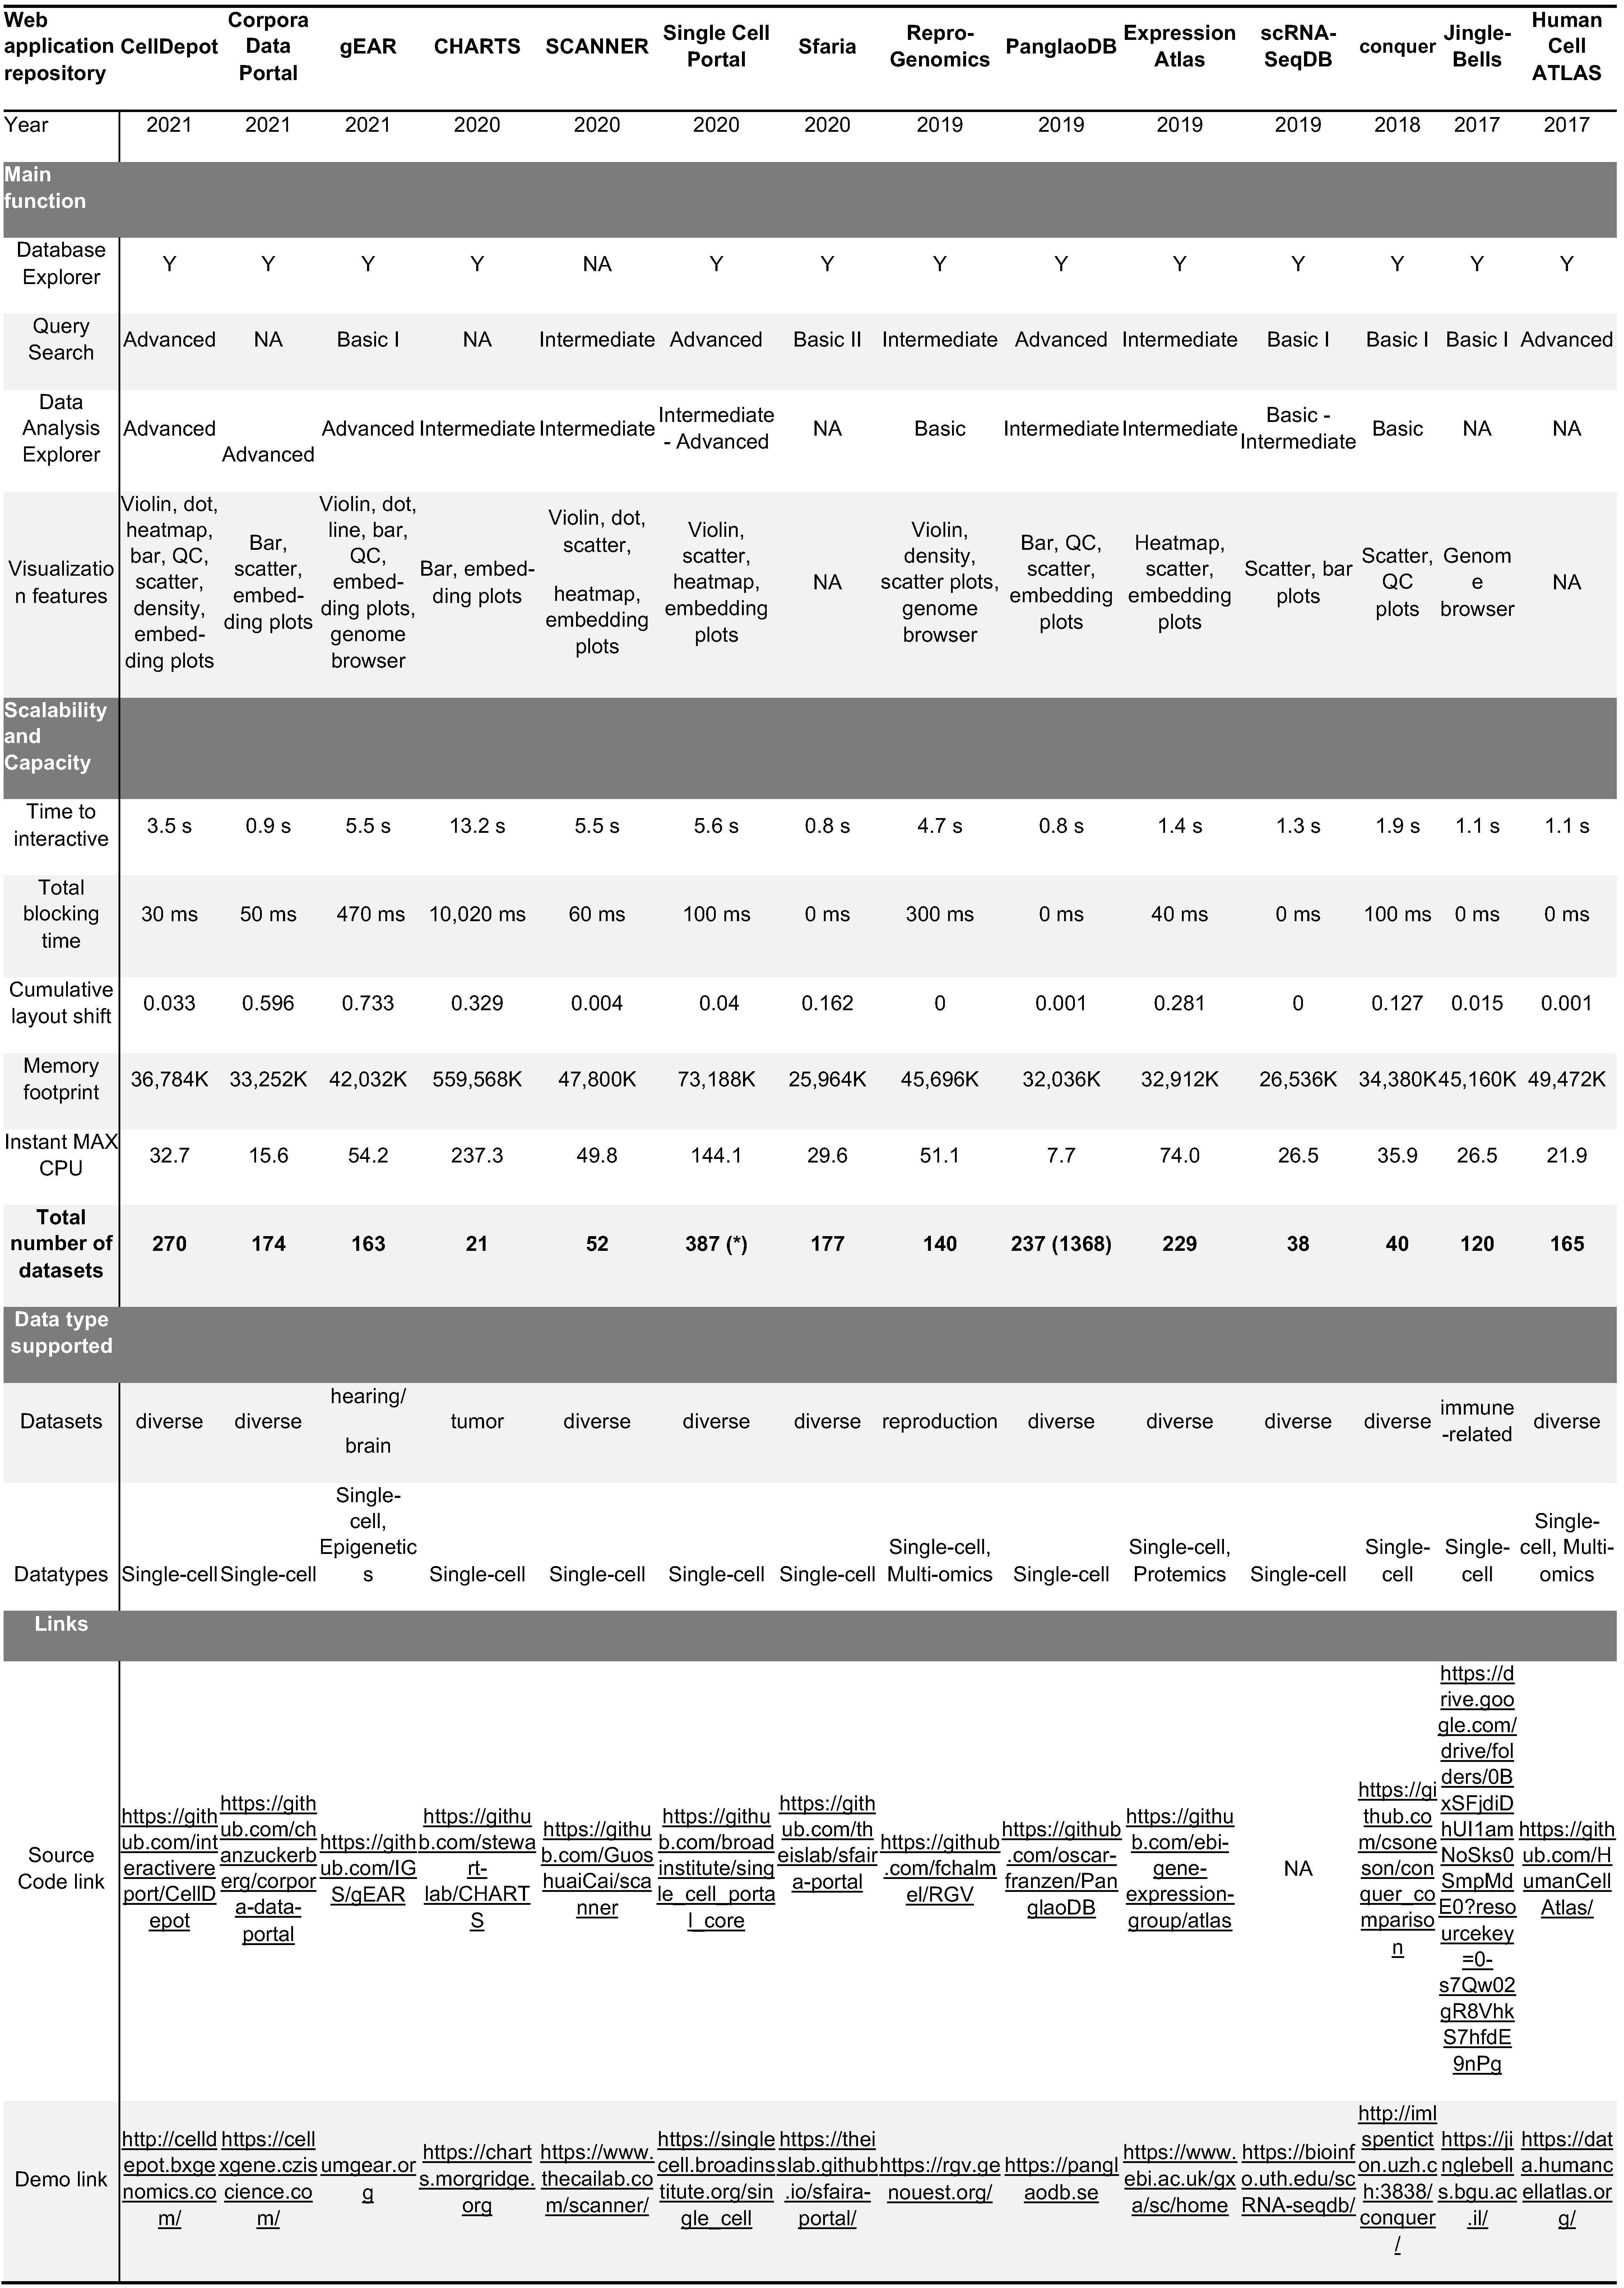
\includegraphics{figures/table_s1.jpg}}

\hypertarget{table-s2---criterion-for-query-search}{%
\section*{\texorpdfstring{\href{https://github.com/interactivereport/CellDepot/blob/gh-pages/bookdown/S2.csv}{Table S2} - Criterion for query search}{Table S2 - Criterion for query search}}\label{table-s2---criterion-for-query-search}}
\addcontentsline{toc}{section}{\href{https://github.com/interactivereport/CellDepot/blob/gh-pages/bookdown/S2.csv}{Table S2} - Criterion for query search}

Table link: \url{https://github.com/interactivereport/CellDepot/blob/gh-pages/bookdown/S2.csv}

\begin{table}
\centering
\begin{tabular}[t]{l|l|l|l}
\hline
Query.Search & Keyword.Search & Multiple.Object.Search & Category.Filters\\
\hline
Basic S2 & Y &  & \\
\hline
Basic II &  &  & Y\\
\hline
Intermediate & Y &  & Y\\
\hline
Advanced & Y & Y & Y\\
\hline
\end{tabular}
\end{table}

\hypertarget{table-s3---criterion-for-data-analysis-explorer}{%
\section*{\texorpdfstring{\href{https://github.com/interactivereport/CellDepot/blob/gh-pages/bookdown/S3.csv}{Table S3} - Criterion for data analysis explorer}{Table S3 - Criterion for data analysis explorer}}\label{table-s3---criterion-for-data-analysis-explorer}}
\addcontentsline{toc}{section}{\href{https://github.com/interactivereport/CellDepot/blob/gh-pages/bookdown/S3.csv}{Table S3} - Criterion for data analysis explorer}

Table link: \url{https://github.com/interactivereport/CellDepot/blob/gh-pages/bookdown/S3.csv}

\begin{table}
\centering
\begin{tabular}[t]{l|l|l|l}
\hline
Data.Analysis.Explorer & Analyze.scRNAseq.Data & Anaylze.Gene.Expression & Customize.Displays\\
\hline
Basic & Y &  & \\
\hline
Intermediate & Y & Y & \\
\hline
Advanced & Y & Y & Y\\
\hline
\end{tabular}
\end{table}

\hypertarget{table-s4---project-metadata-captured-in-celldepot}{%
\section*{\texorpdfstring{\href{https://github.com/interactivereport/CellDepot/blob/gh-pages/bookdown/S4.csv}{Table S4} - Project metadata captured in CellDepot}{Table S4 - Project metadata captured in CellDepot}}\label{table-s4---project-metadata-captured-in-celldepot}}
\addcontentsline{toc}{section}{\href{https://github.com/interactivereport/CellDepot/blob/gh-pages/bookdown/S4.csv}{Table S4} - Project metadata captured in CellDepot}

Table link: \url{https://github.com/interactivereport/CellDepot/blob/gh-pages/bookdown/S4.csv}

\begin{table}
\centering
\begin{tabular}[t]{l|l|l}
\hline
General.Category & Expected.Variable.Type & Description\\
\hline
Annotation Groups & String & categorical  features from h5ad file\\
\hline
Cell Count & Integer & numbers of cell in study\\
\hline
Actions & Link & three options: 1) Study summary information; 2) Data visualization and analysis; 3) Update project information\\
\hline
Custom Accession & String & Customized accession name for individual project\\
\hline
Description & String & Additional information\\
\hline
DOI & Link & Digtial Object Identifier\\
\hline
File Name & String & h5ad file name\\
\hline
File Size & Integer & size of h5ad file\\
\hline
Gene Count & Integer & numbers of gene in study\\
\hline
Name & Link & project name\\
\hline
Notes & String & study notes\\
\hline
PMC ID & Link & \\
\hline
Publication Title &  & \\
\hline
PubMed ID & Link & \\
\hline
Speices & String & \\
\hline
URL & Link & \\
\hline
Year & String & \\
\hline
\end{tabular}
\end{table}

\hypertarget{SITutorial}{%
\chapter{Supplemental Tutorial}\label{SITutorial}}

CellDepot is a scRNA-seq data portal consisting of a relational database management system, a graphical query builder, and data visualization tools, which can be accessed via the link, \url{http://celldepot.bxgenomics.com} for public datasets or a link to private installation, e.g., \url{http://go.biogen.com/CellDepot} for Biogen internal data collection. This is the supplemental tutorial providing detailed instructions. Clicking on a figure will bring up the enlarged view.

\href{figures/S1.jpg}{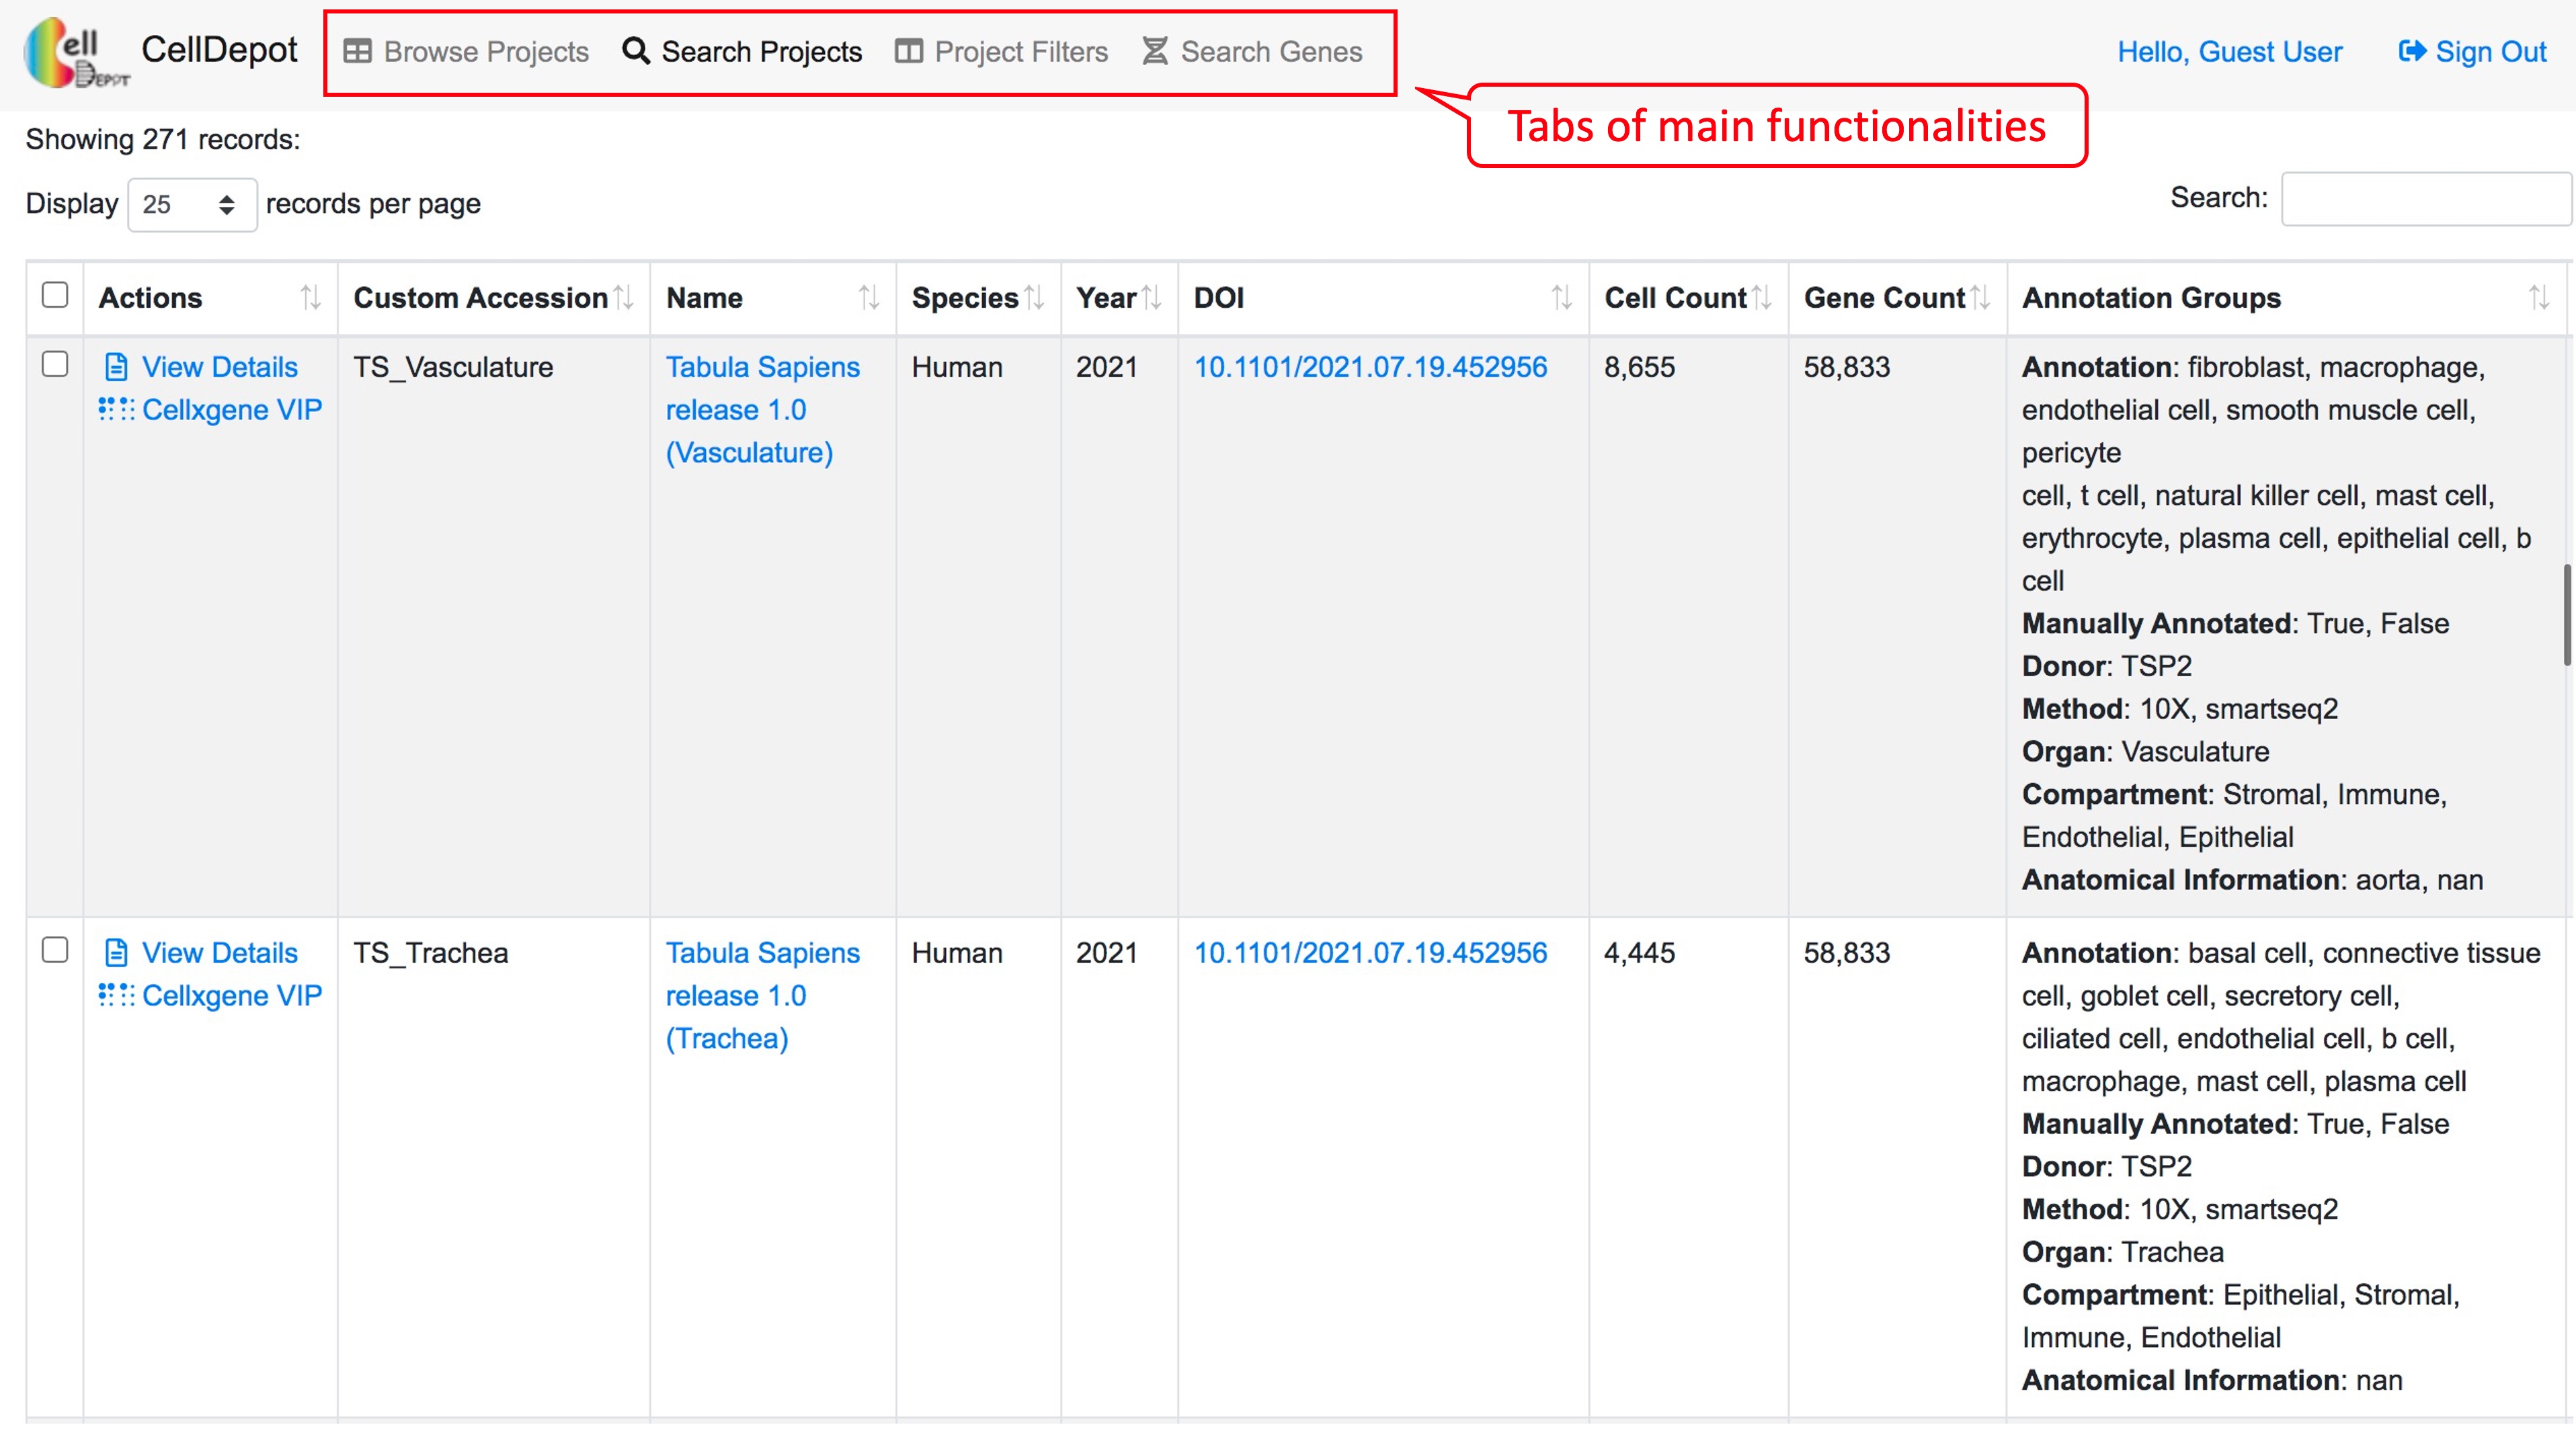
\includegraphics{figures/S1.jpg}}

Figure S1. CellDepot Homepage. Functions designated to different user roles are highlighted in red callout boxes.

The interface contains multiple tabs at the top of the homepage, which correspond to major functionalities of CellDepot. All users can explore the existing datasets loaded in the public CellDepot for visualization and analysis while only admin users can upload datasets to a CellDepot instance, public or private.

\hypertarget{browse-projects}{%
\section{Browse Projects}\label{browse-projects}}

Users can customize columns to be displayed by clicking on the green `Column Settings' button. In addition, all or selected entries could be exported in CSV format. A quick search box is provided on the top-right corner of the table while building a complex query is exemplified in Figure S3 (\ref{search}).

\href{figures/S2.jpg}{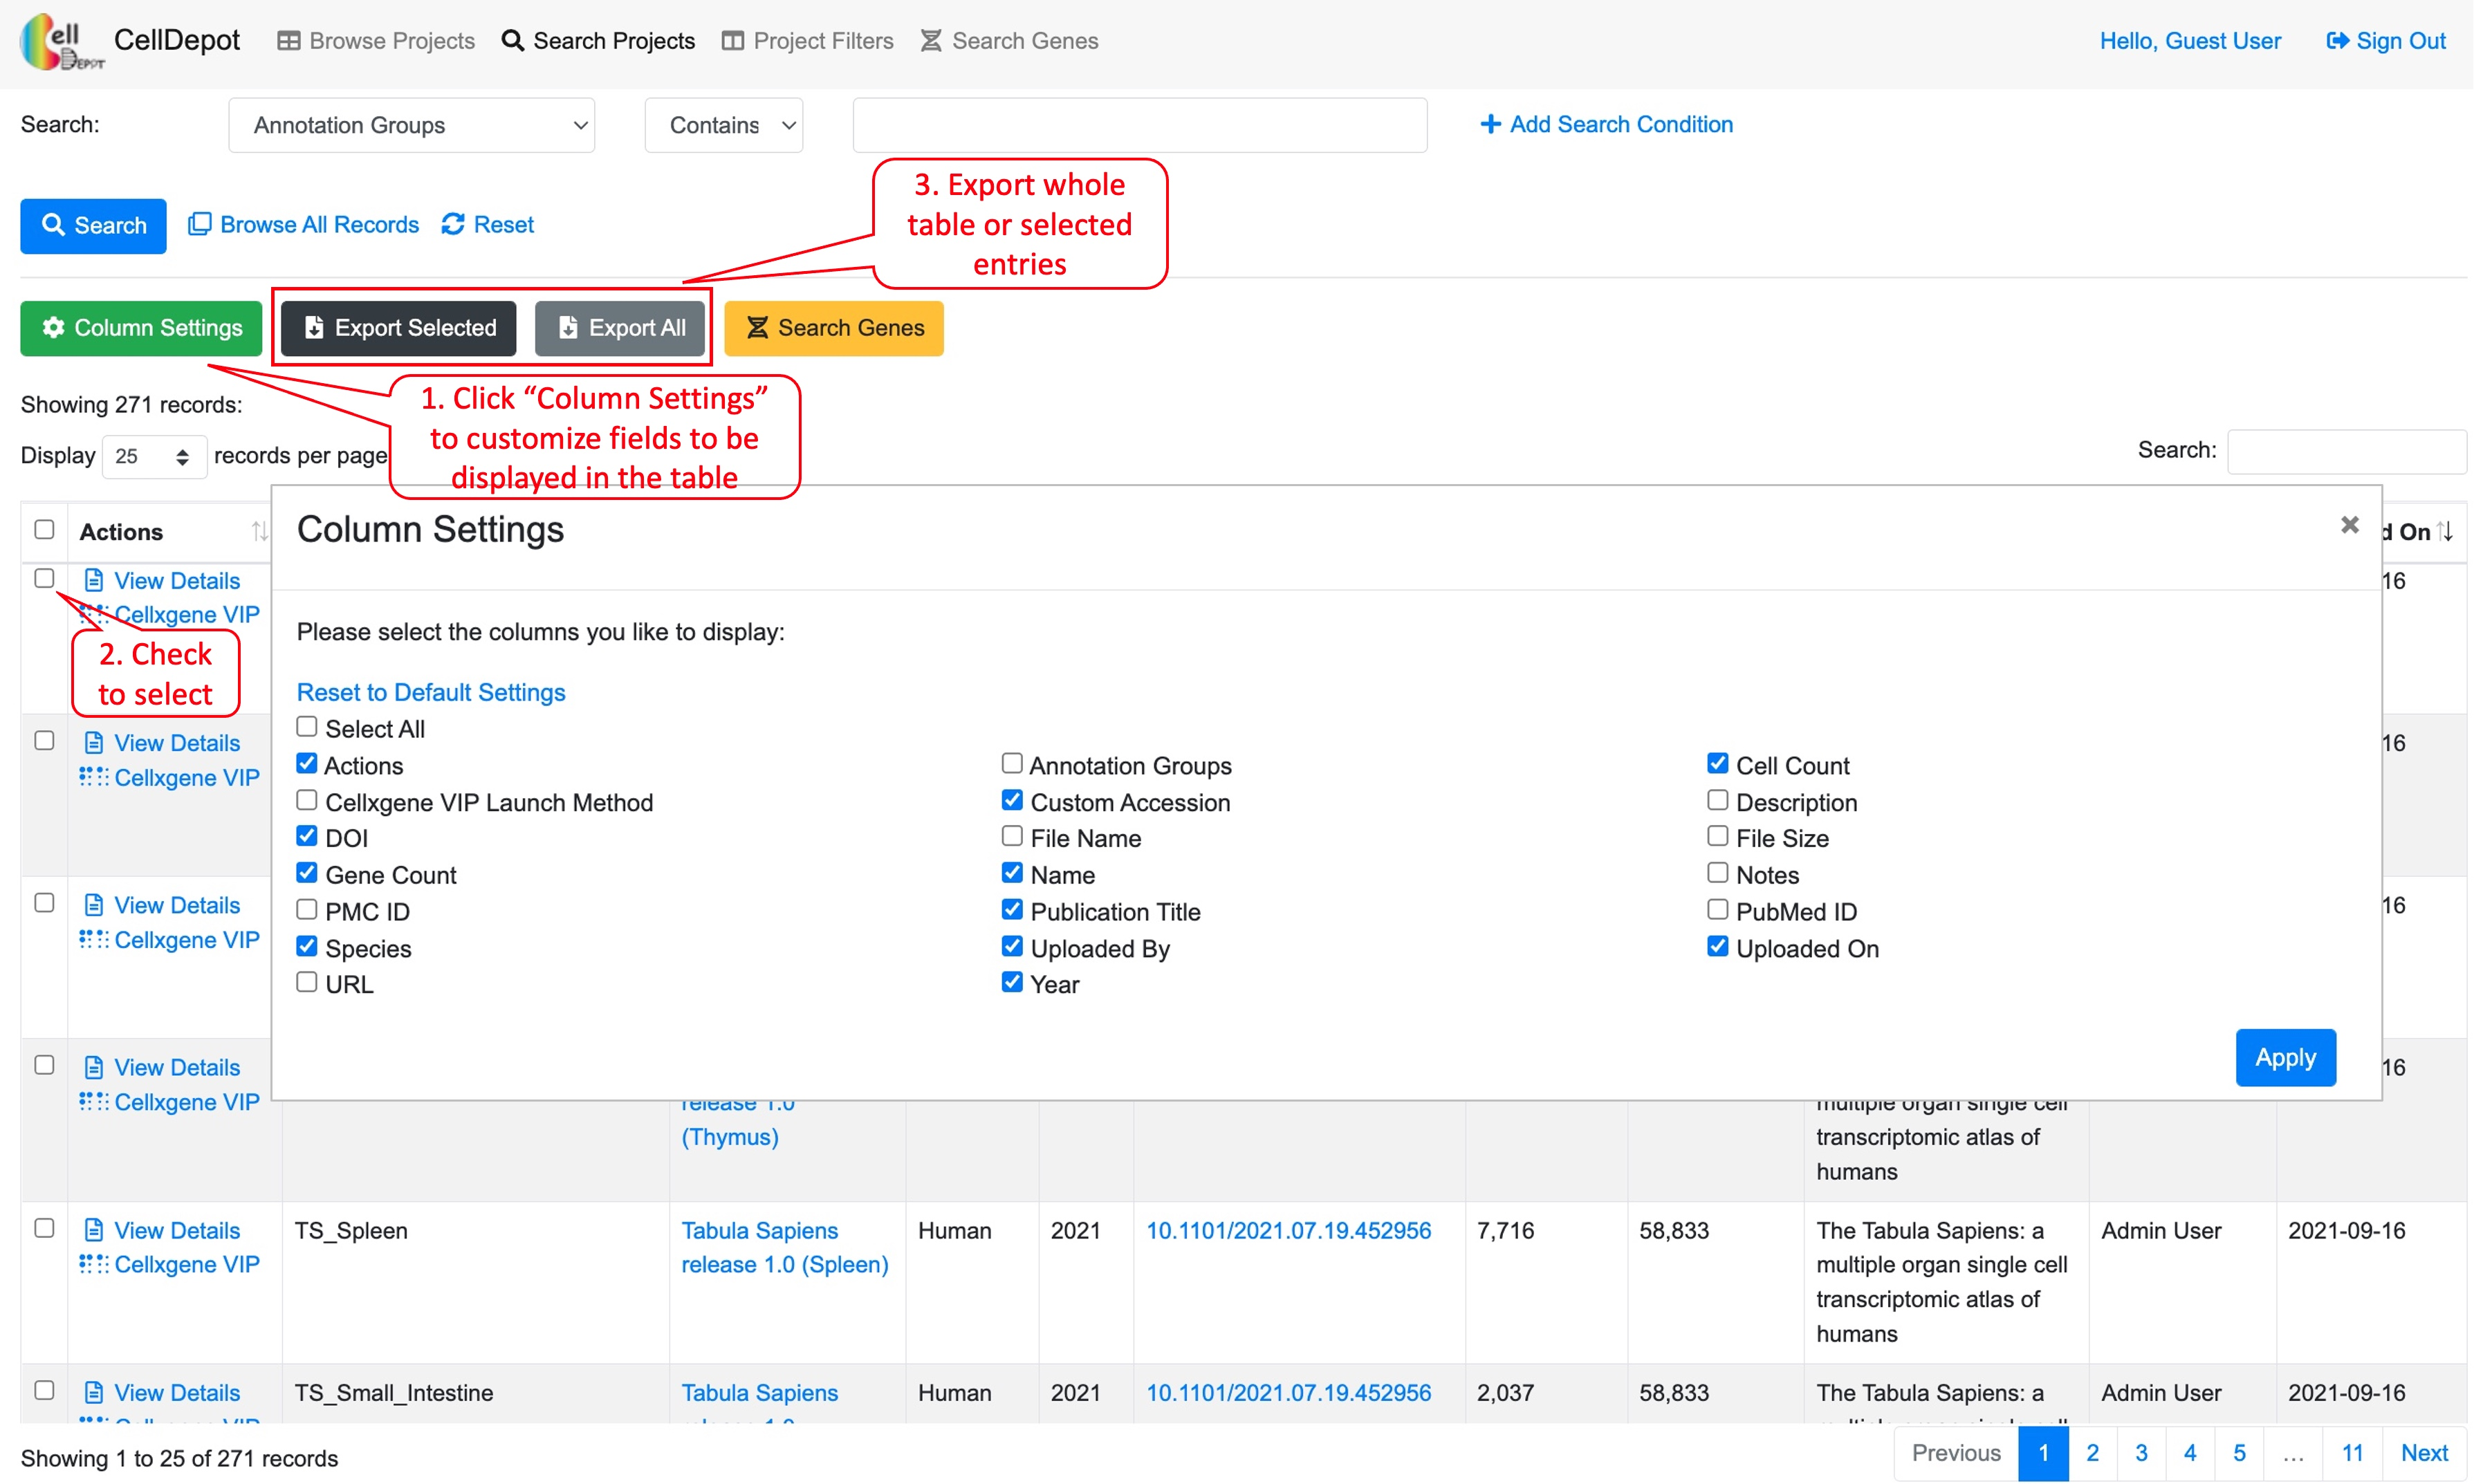
\includegraphics{figures/S2.jpg}}
Figure S2. Browsing projects in a personalized view.

\hypertarget{search}{%
\section{Search Projects}\label{search}}

This function allows users to search projects of interest, which can be accessed through the homepage as well. Users can search projects by 17 attributes in multiple logic conditions: annotation groups, cell count, cellxgene VIP launch method, Custom accession, description, DOI, file name, file size, gene count, name, notes, PMC ID, Publication Title, PubMed ID, Species, URL, and/or Year.

\href{figures/S3.jpg}{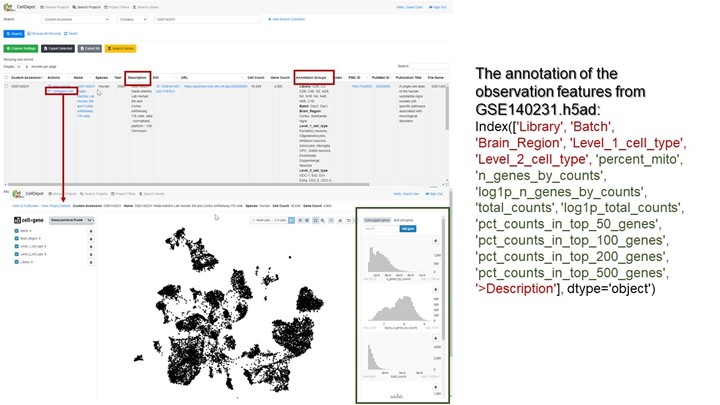
\includegraphics{figures/S3.jpg}}
Figure S3. Workflow of searching projects by using the graphical multi-logic, multi-condition query builder. Six datasets are identified when searching by `Species is Human' and `Annotation Group contains Neuron'.

\hypertarget{project-filters}{%
\section{Project Filters}\label{project-filters}}

This function lists the filtered datasets simply based on AND logic operation of checked items under various categories. It is a friendly feature for first-time users as they may not be familiar with the design of the database to construct more complex query.

\href{figures/S4.jpg}{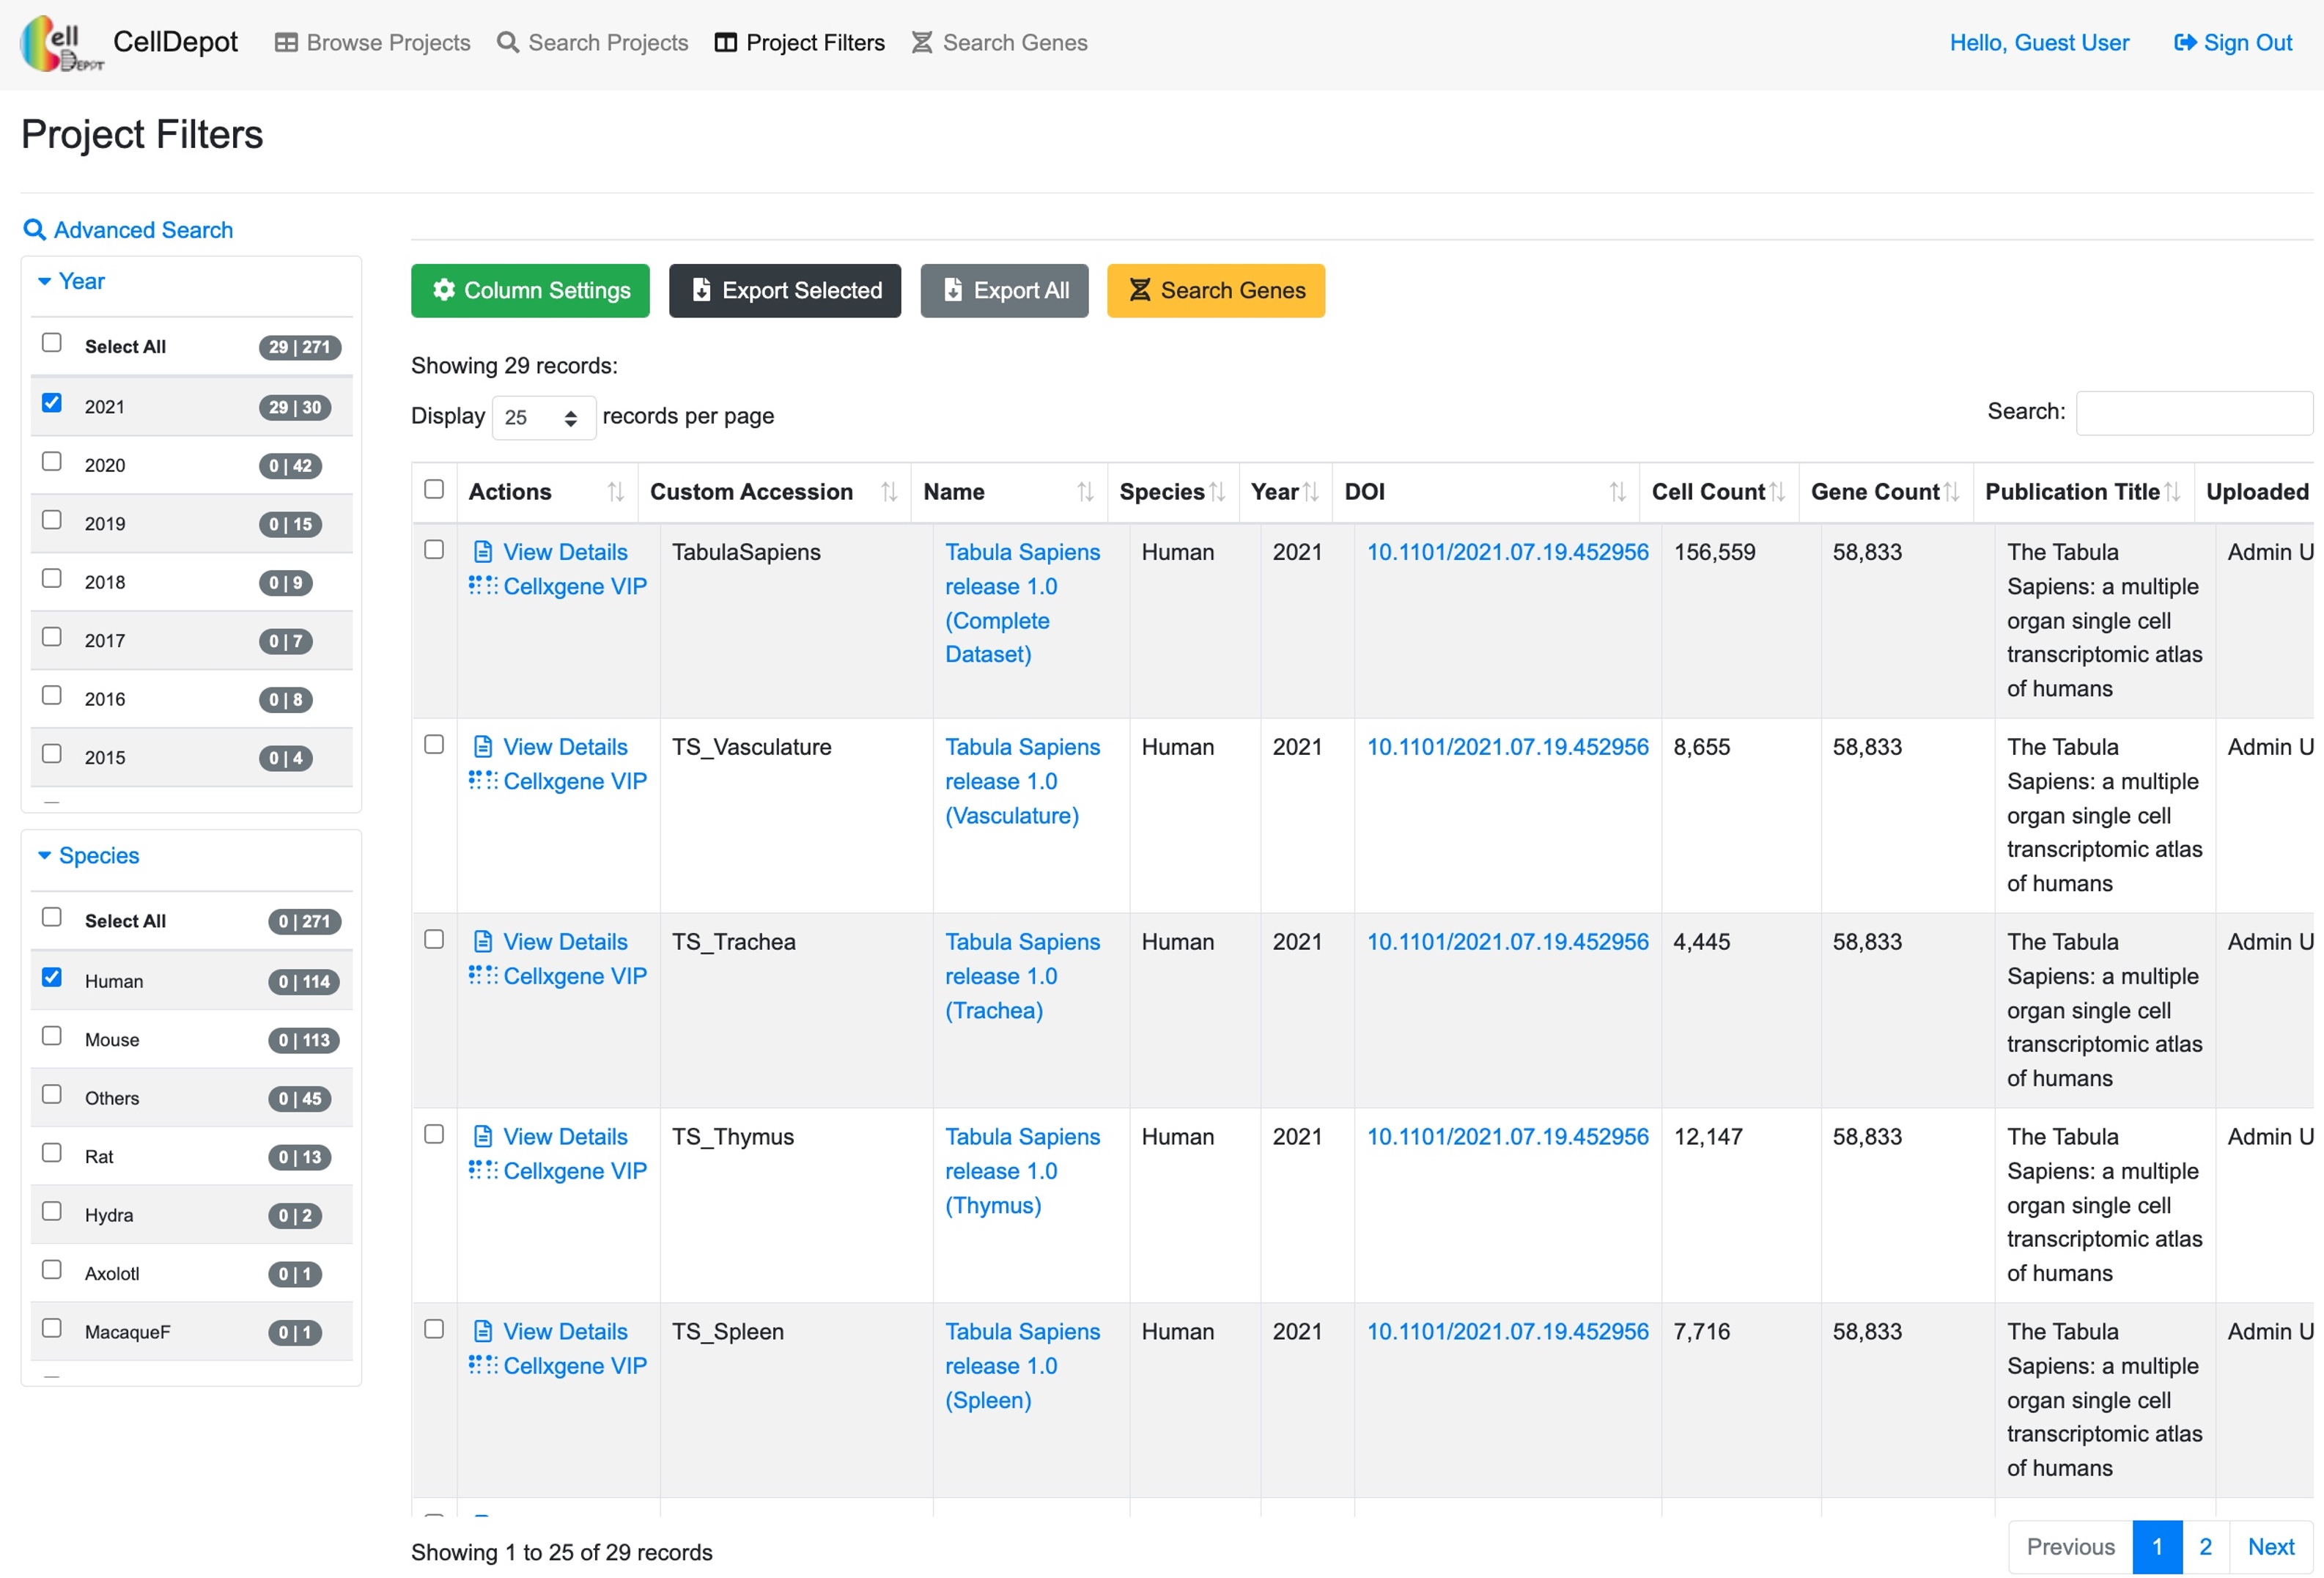
\includegraphics{figures/S4.jpg}}
Figure S4. The `Project Filters' page. 29 records are identified by filtering criteria of `Year' equaling 2021 and `Species' being human.

\hypertarget{visualize-datasets}{%
\section{Visualize Datasets}\label{visualize-datasets}}

\hypertarget{view-details}{%
\subsection{View Details}\label{view-details}}

The dataset information consists of project summary and annotation groups. The project summary is provided by admin users when uploading projects while annotation groups are retrieved from uploaded h5ad files.

\href{figures/S5.jpg}{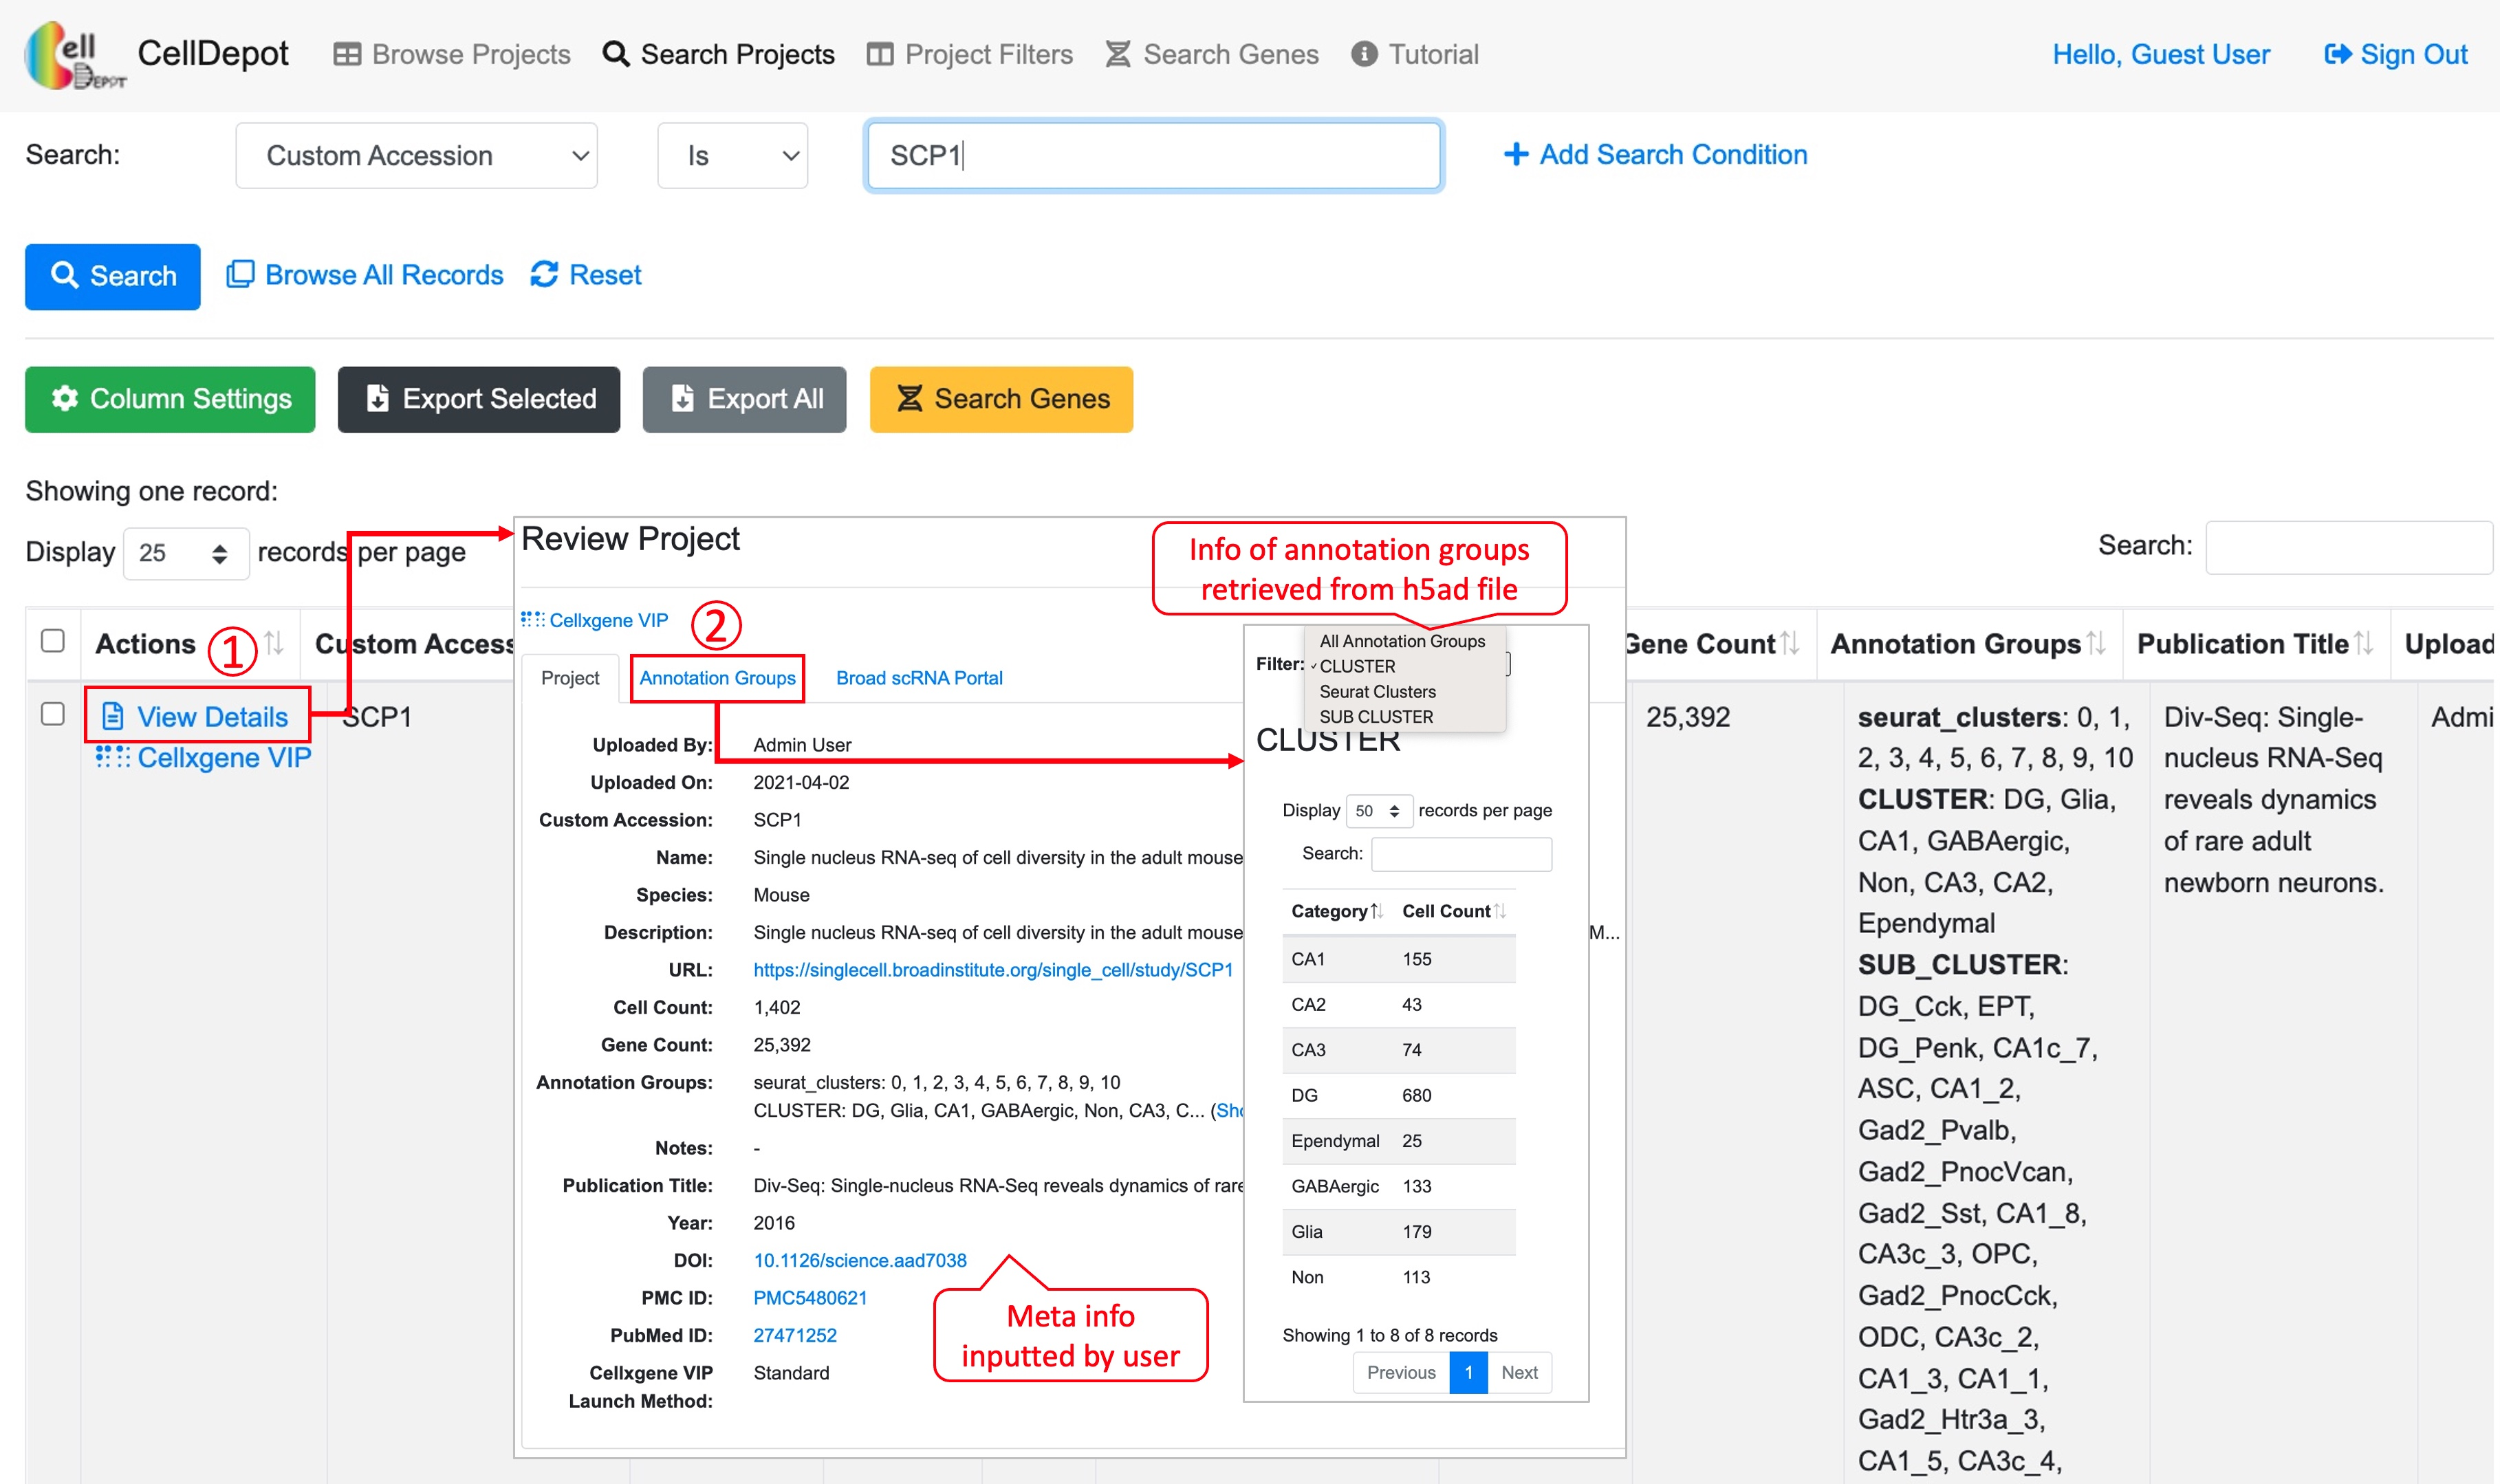
\includegraphics{figures/S5.jpg}}
Figure S5. How to view details of a dataset. Steps are outlined by red circled numbers.

\hypertarget{figures6}{%
\subsection{Data Visualization and Analysis by cellxgene VIP}\label{figures6}}

CellDepot is not only a database management system, but also a web portal for visualizing and analyzing scRNA-seq datasets through embedded cellxgene VIP tool. By clicking `cellxgene VIP' to access functional modules on the menu, users can perform advanced data visualization and analysis. To learn how to use cellxgene VIP, please go to \url{https://interactivereport.github.io/cellxgene_VIP/tutorial/docs/how-to-use-cellxgene-vip.html}.

\href{figures/S6.jpg}{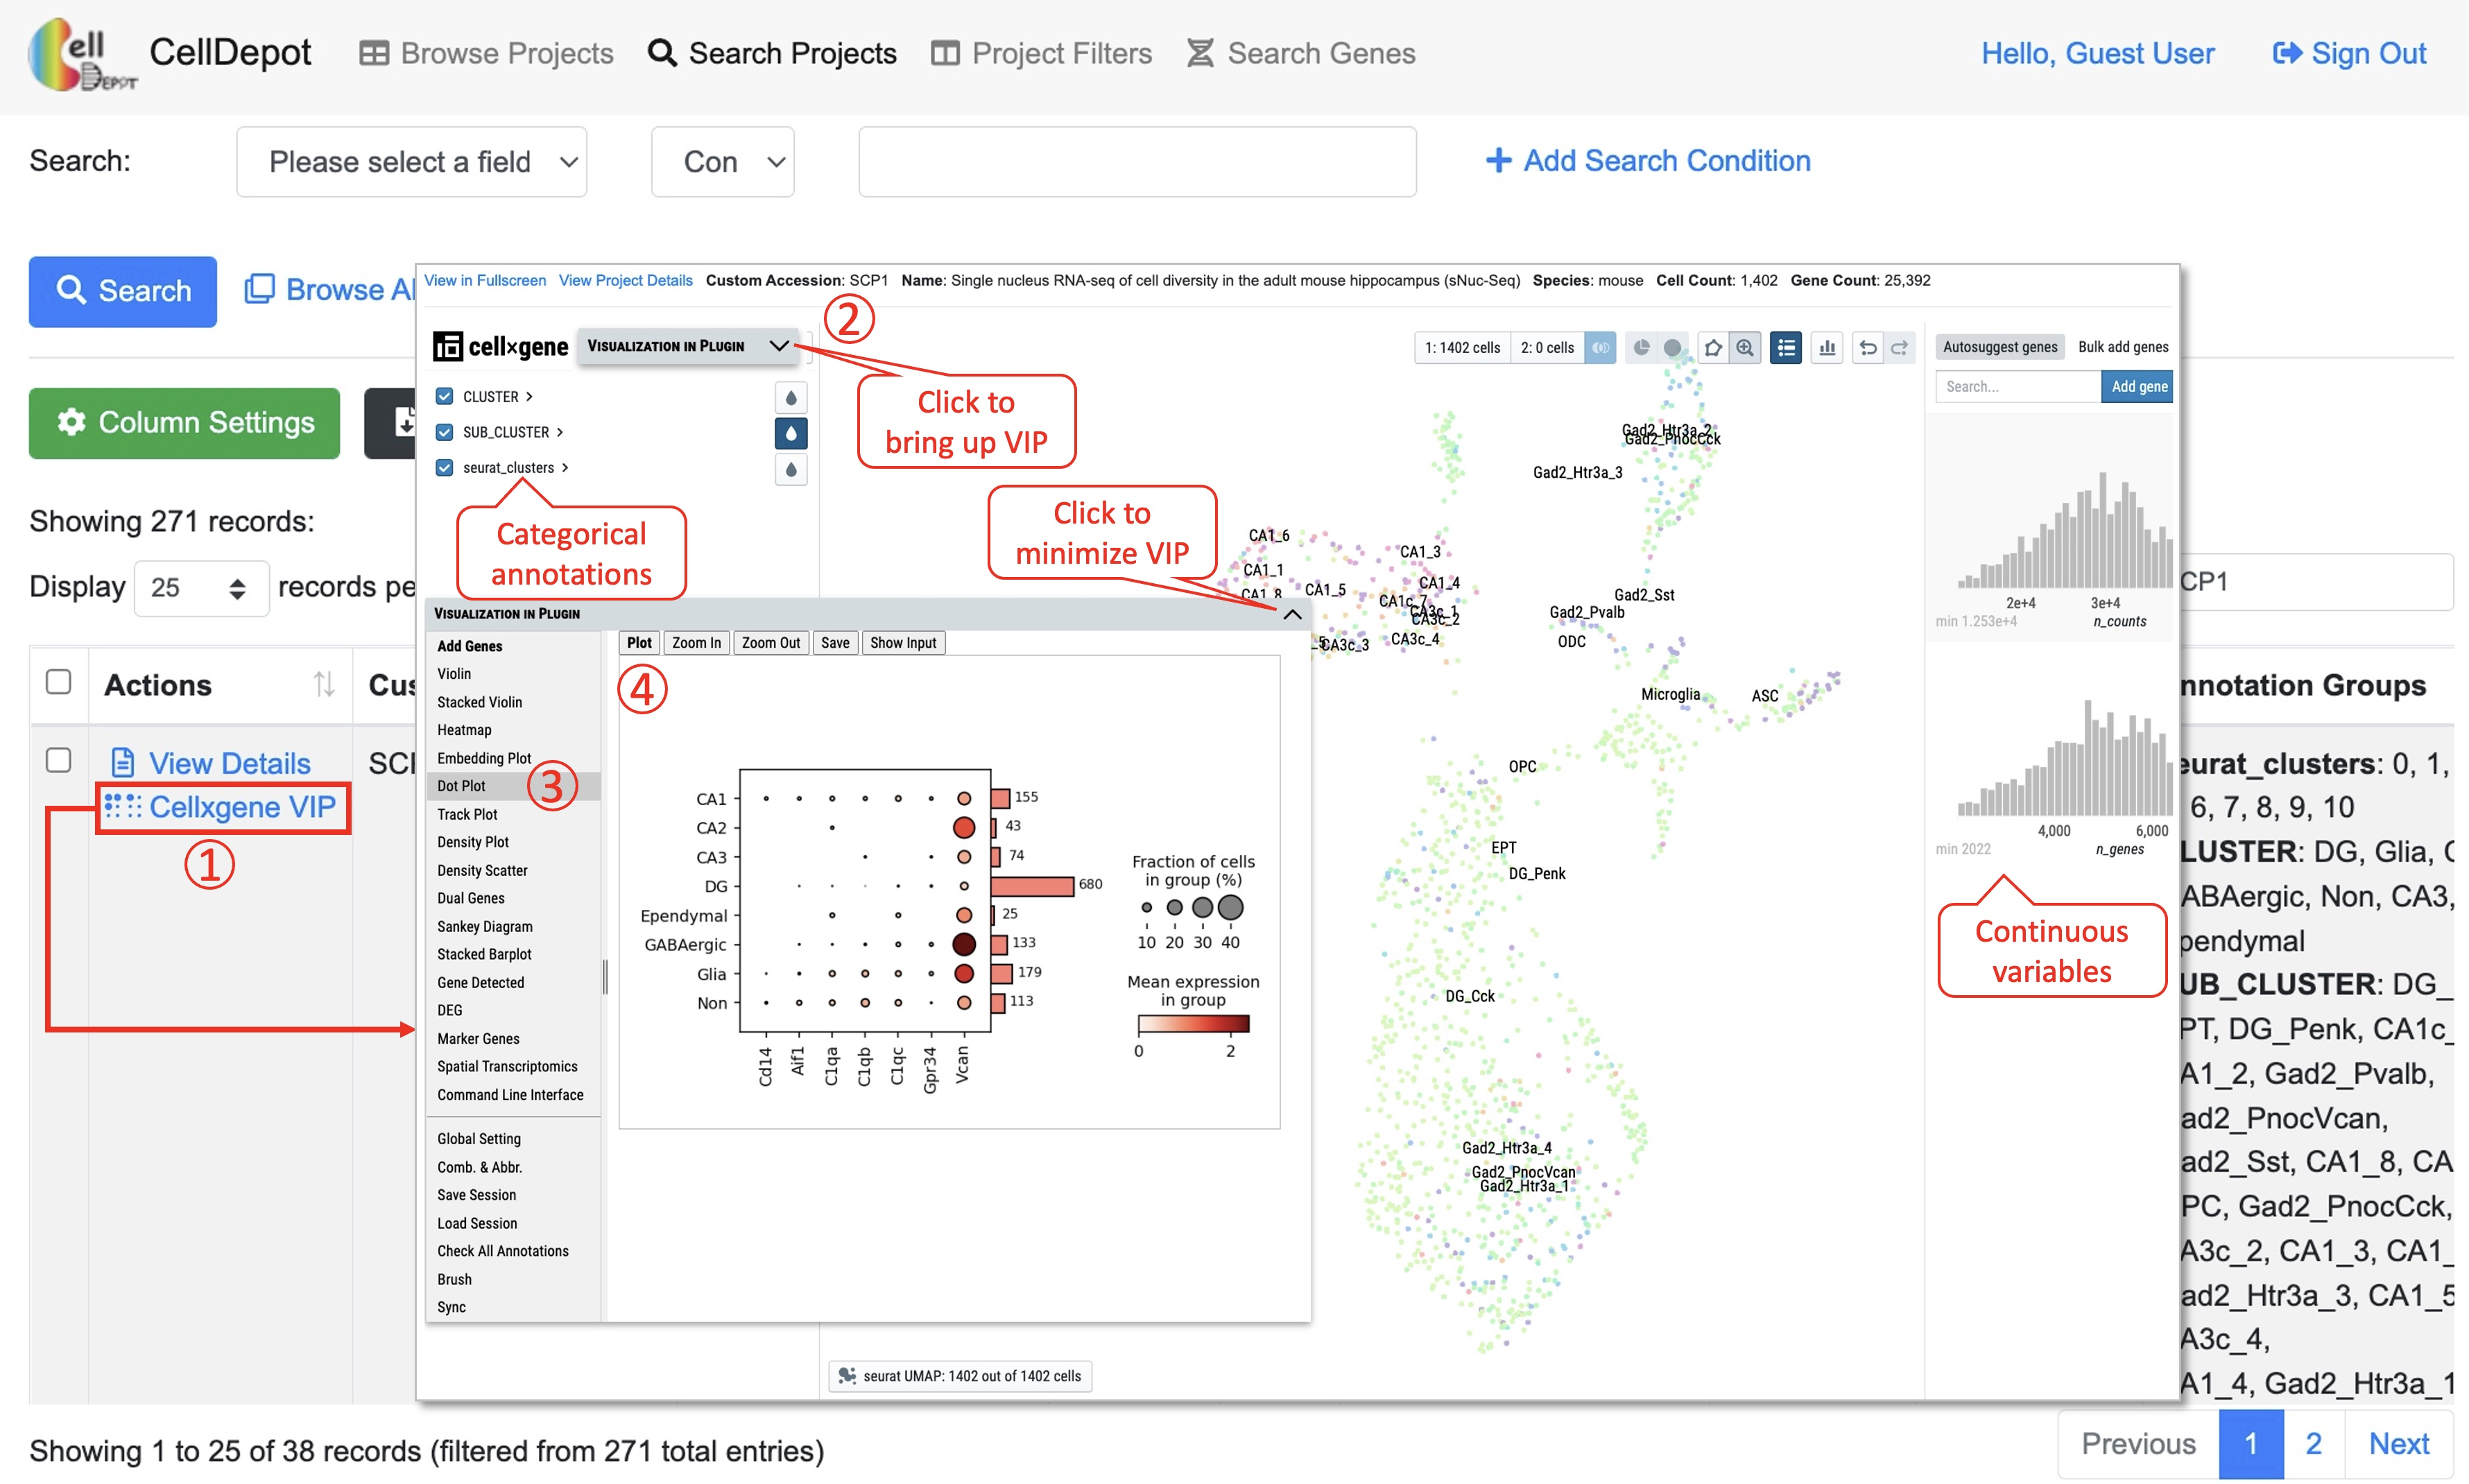
\includegraphics{figures/S6.jpg}}
Figure S6. Visualization and analysis of a scRNA-seq dataset by cellxgene VIP.

\hypertarget{case-study-1}{%
\subsection{Case Study 1}\label{case-study-1}}

Exploration and visualization of differentially expressed genes (DEGs) between two types of cells.

As shown in Figure S7a, two types of cells, Astrocytes (1036 cells) and Oligodendrocytes (4417 cells) are selected. By running differential gene expression analysis with one of the built-in statistical methods such as Welch's t-test, we detected 1578 (DEGs), including 715 up-regulated and 853 down-regulated genes in astrocytes compared to oligodendrocytes (Figure S7a). The expression of the top four DEGs among the cell types indicates that gene MBP, ST18 and RNF220 are expressed explicitly in oligodendrocytes, while gene PITPNC3 is expressed mainly in astrocytes and endothelial cells (Figure S7b).

\href{figures/S7.jpg}{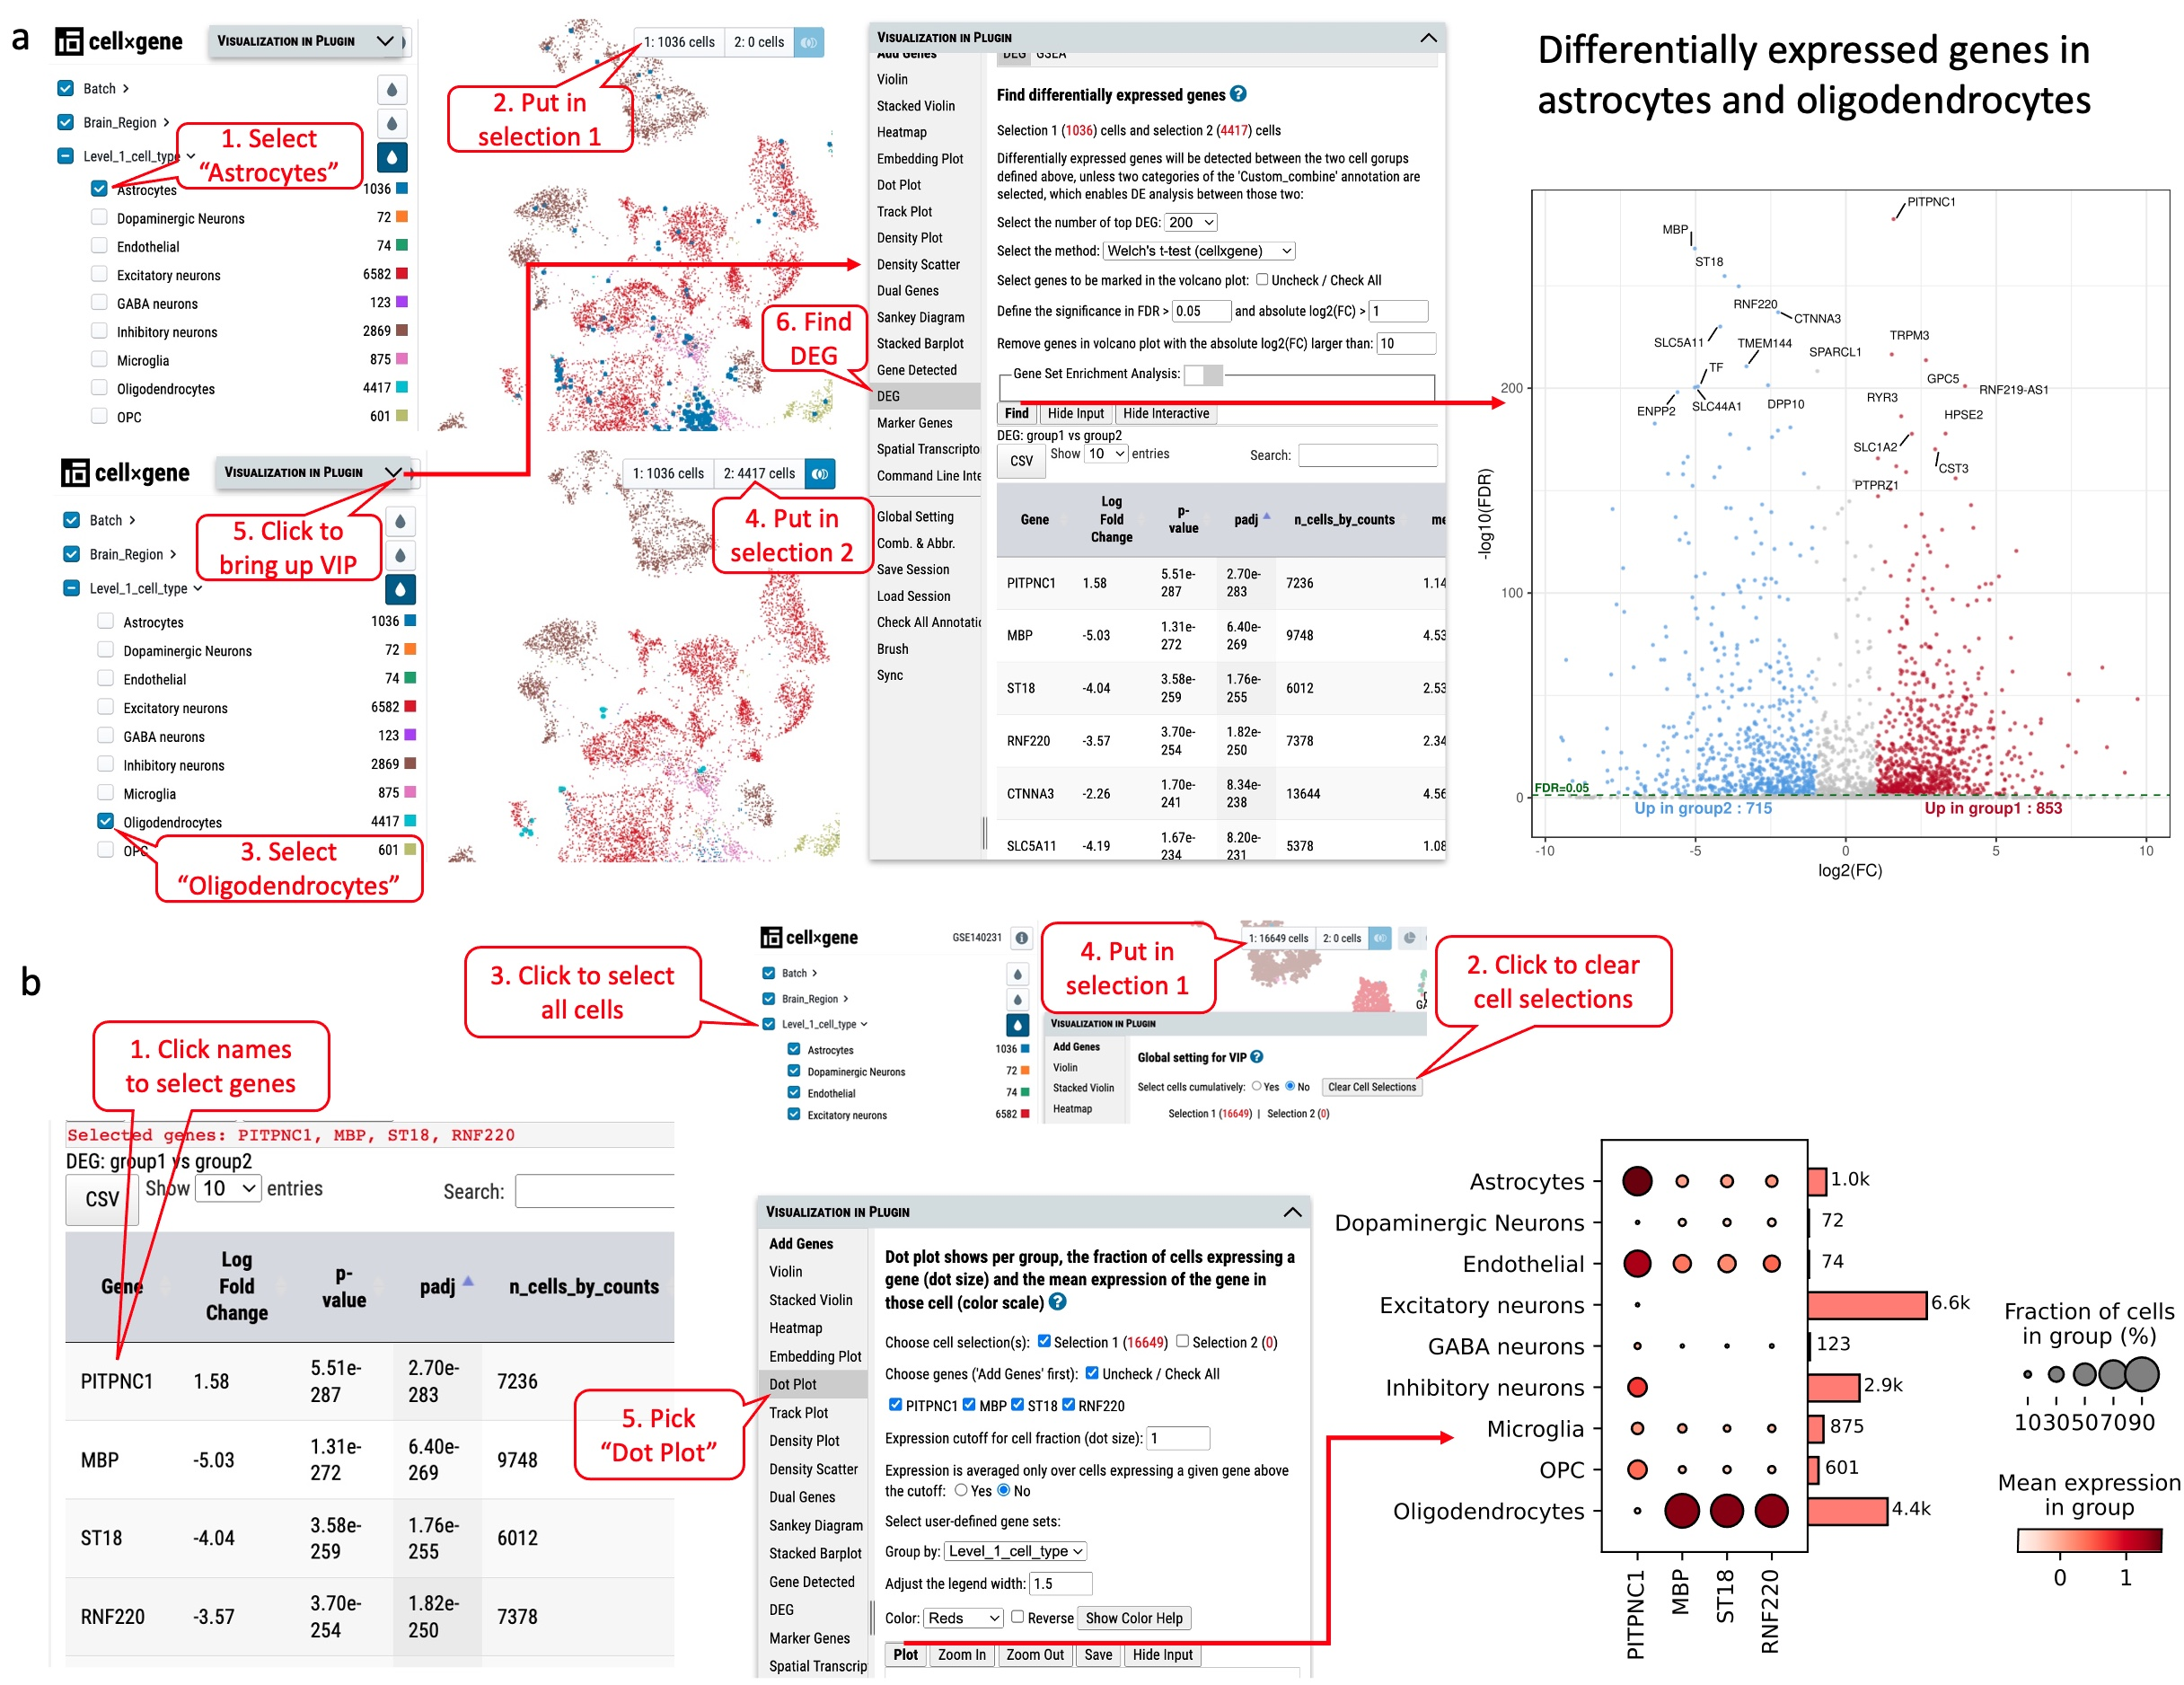
\includegraphics{figures/S7.jpg}}
Figure S7. Exploration of differentially expressed genes in dataset GSE140231 through cellxgene VIP. (a) Identifying differentially expressed genes in astrocytes and oligodendrocytes. (b) The expression of top four genes in various cell types as shown in dot plot.

\hypertarget{search-genes}{%
\section{Search Genes}\label{search-genes}}

This tab allows searching on genes of interest with the expression cutoff. The search outcome provides users a list of projects in which genes of interest are expressed above the cutoff. Each project displays a link to project page and a plot if applicable. This plot can be either a violin plot or dot plot showing the gene expression level in a selected annotation group. Further, under ``Advanced Options'', users can define the range of expression color scale and the percentage represented by the largest dot to have expression data from various projects plotted in a unified manner.

\href{figures/S8.jpg}{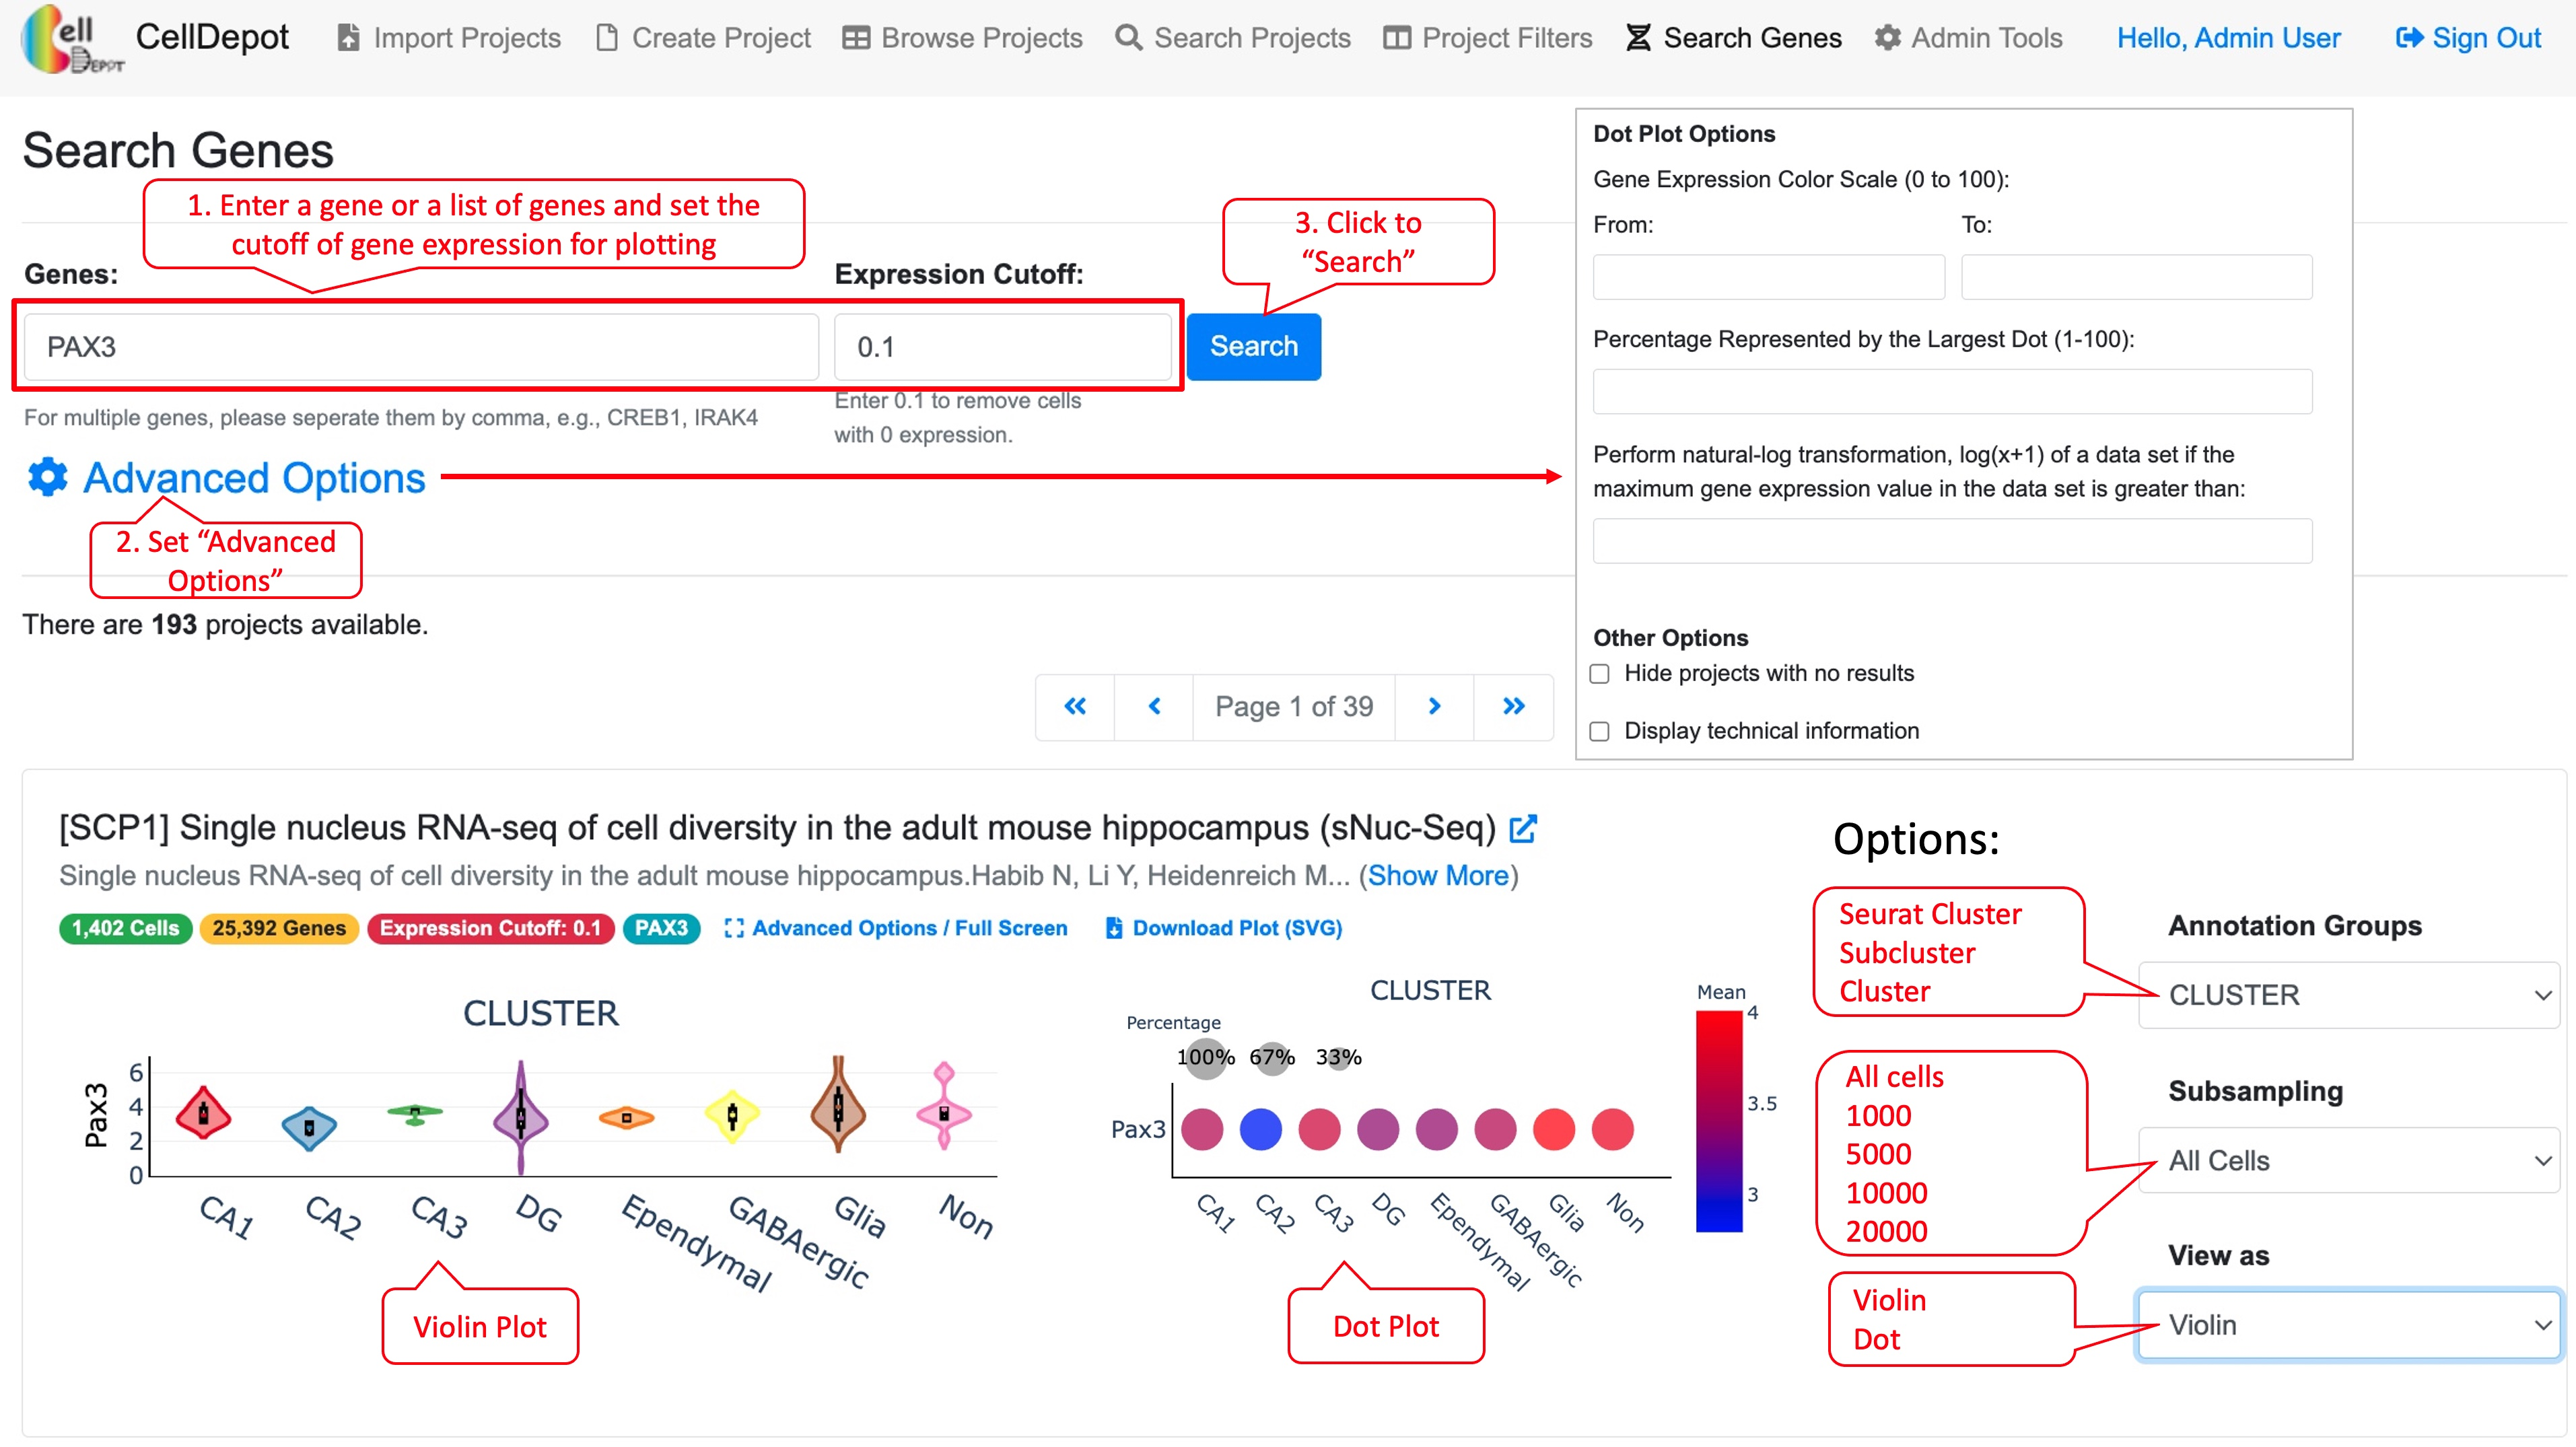
\includegraphics{figures/S8.jpg}}
Figure S8. Steps to find gene expression level of a gene in projects under `Search Genes' tab. The final plot can be customized by available options listed in red callout boxes on the left side.

\hypertarget{case-study-2}{%
\subsection{Case Study 2}\label{case-study-2}}

Cross-project comparison of skeletal muscle marker genes PAX3, PAX7, PITX2, MYF5, MYF6, MYOD1, MYOG, NEB, and MYH3 among the datasets whose species is human and cell type is myogenic.

\href{figures/s9.jpg}{\includegraphics{figures/s9.jpg}}
Figure S9. Workflow of conducting the cross-project comparison of a list of genes among the selected datasets.

\hypertarget{import}{%
\section{Import Projects}\label{import}}

The functionality is limited to admin users. To upload new projects to CellDepot database in batch, two types of files are required: 1) .h5ad files and 2) project information file in CSV (Comma Separated Values) format. First, the prepared h5ad files are required to be copied to a folder defined in the configuration file, e.g., /data/celldepot/all\_h5ad\_files/. Afterwards, admin users navigate to the CellDepot home page, click `Import Projects' at the top menu, then `Download Example File' to fill in meta information of datasets into the downloaded template for submission. In addition, there are two cellxgene VIP launch modes to chosen from, `Standard' and `Preload in Memory'. `Standard' mode is for infrequently used datasets while `Preload in Memory' should be selected to speed up loading and responding time of frequently used large datasets.
After the metadata file is uploaded, CellDepot will automatically convert the dataset to CSC format if needed through a cron job (\ref{cron}). To explore the detail of imported datasets, users can enter `Browse Projects' page and then search these datasets by user assigned `Custom Accession' identifiers.

\href{figures/S10.jpg}{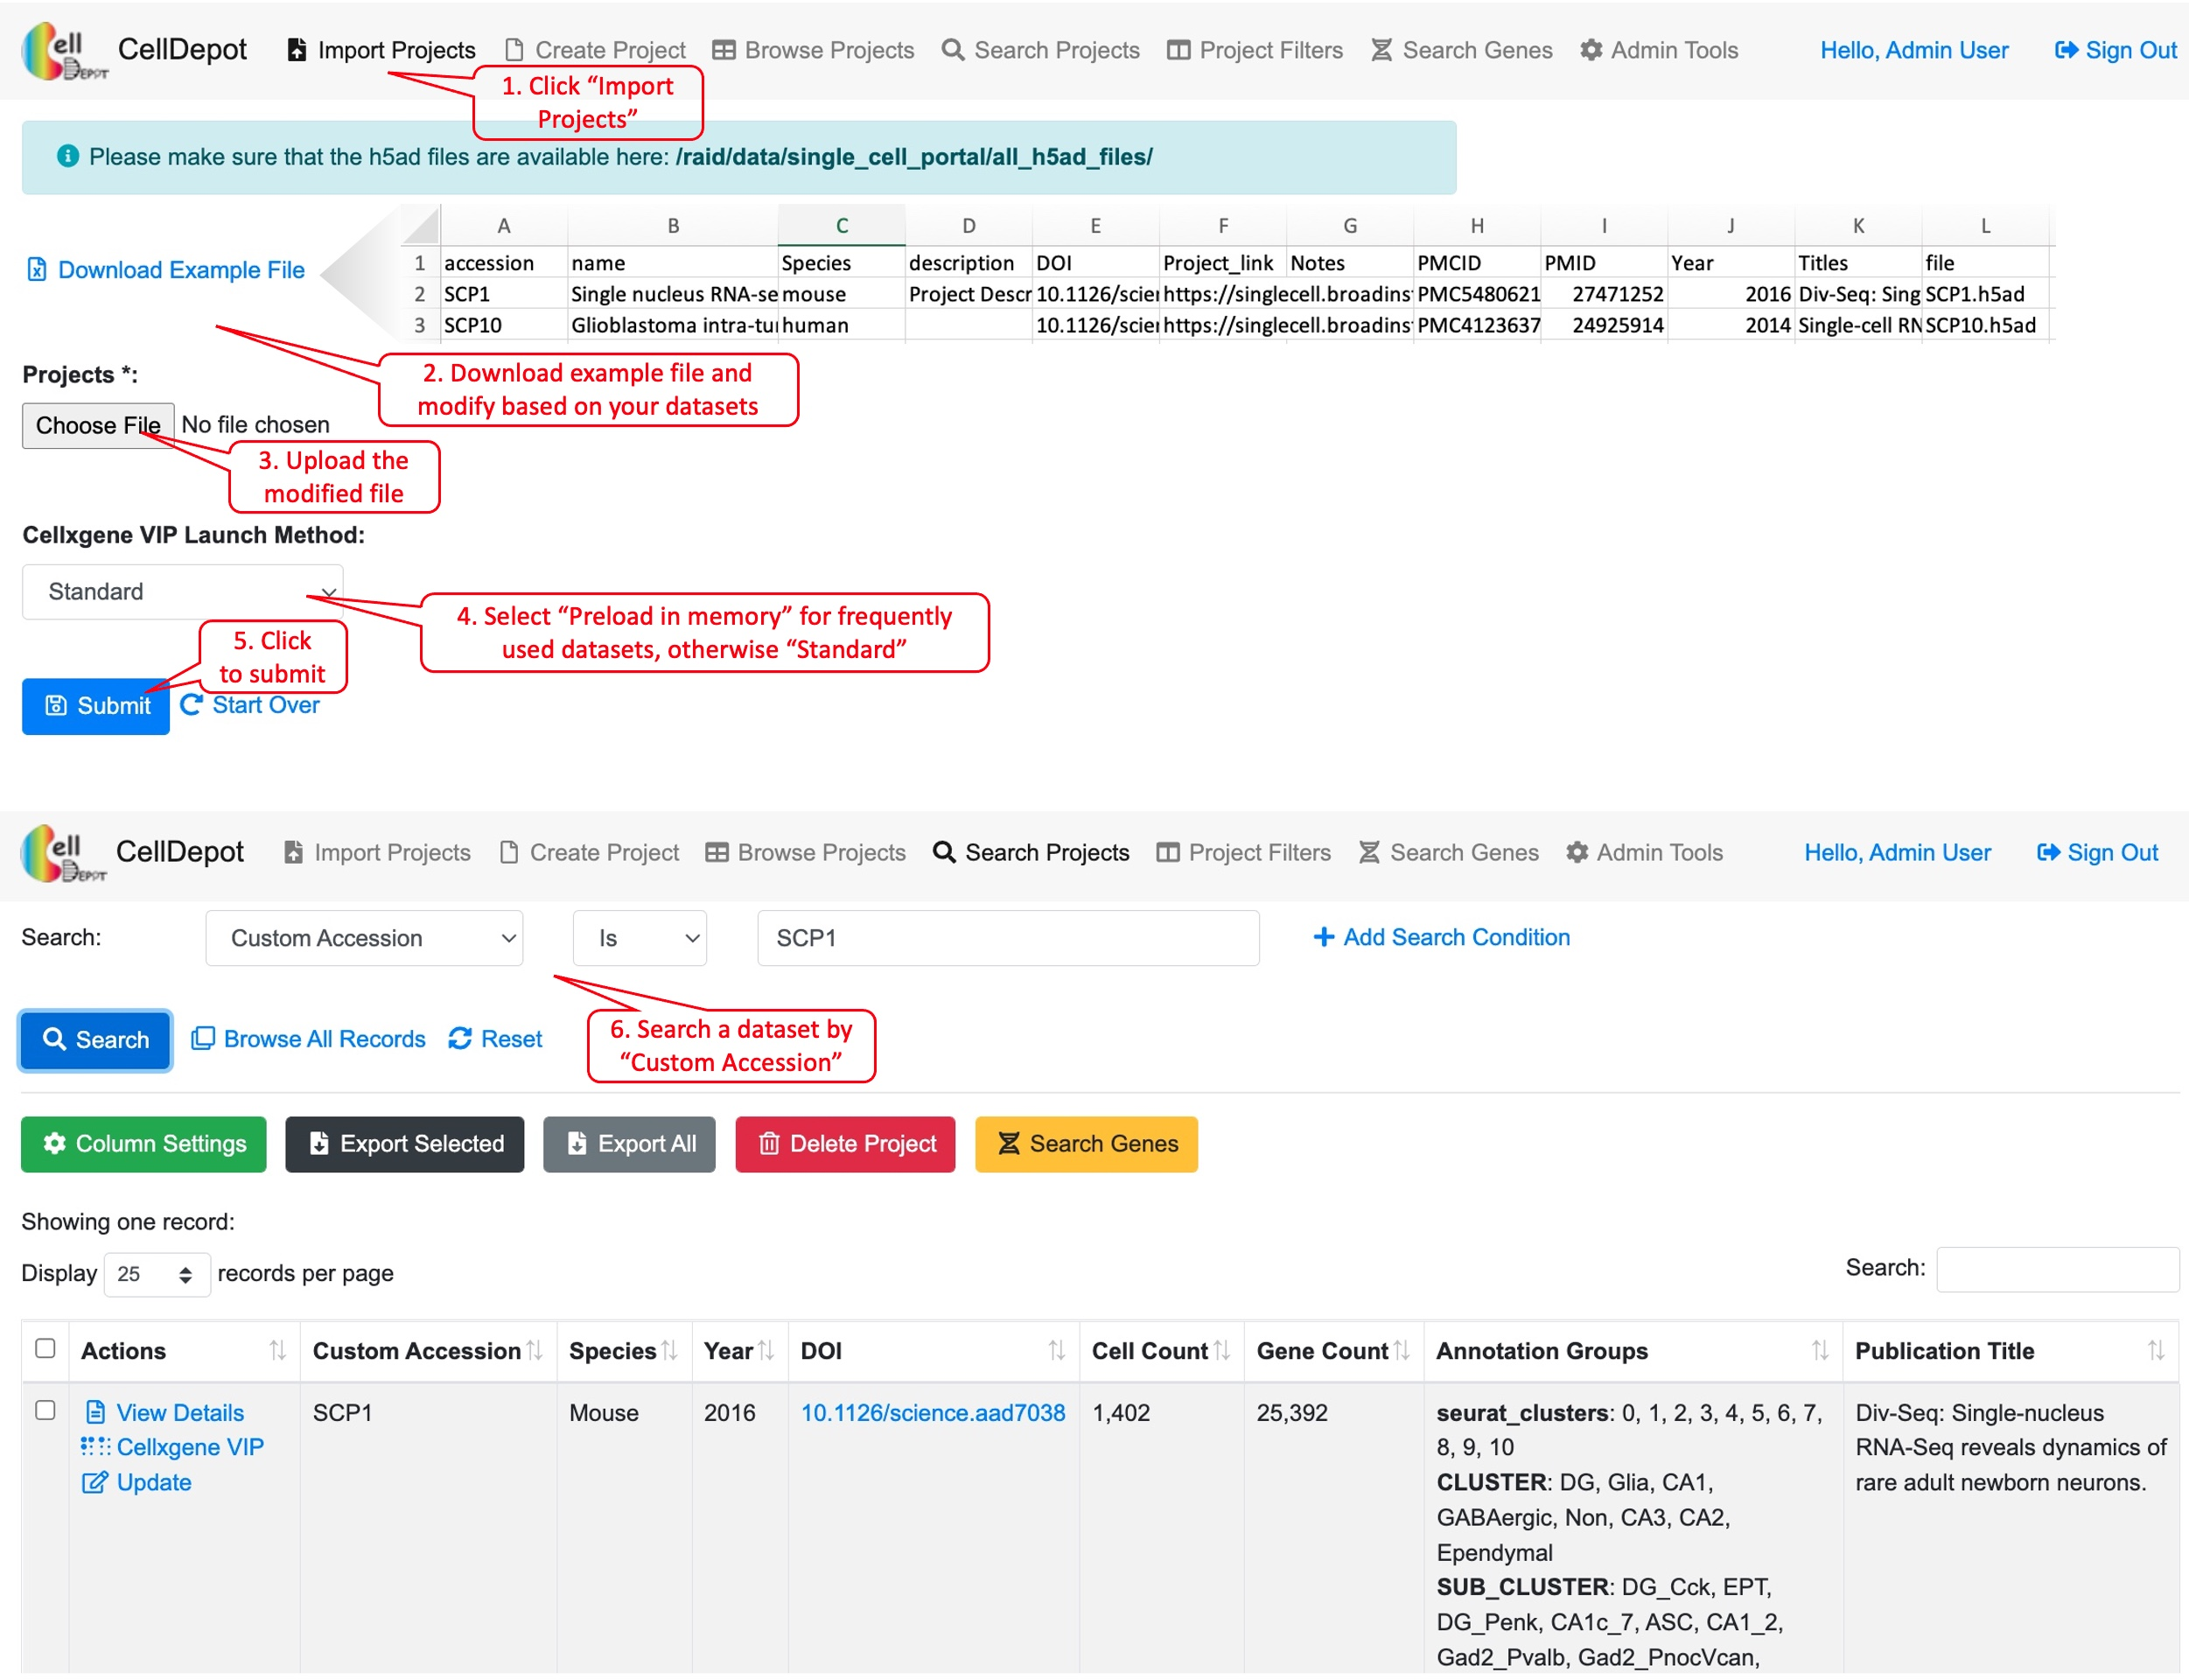
\includegraphics{figures/S10.jpg}}
Figure S10. Workflow of how to import new datasets.

\hypertarget{create-project}{%
\section{Create Project}\label{create-project}}

Besides batch uploading under ``Import Projects'' tab, admin user can use the online form under this tab to submit information of a project.

\hypertarget{update-a-project}{%
\section{Update a Project}\label{update-a-project}}

Project information including launch mode can be modified by admin users by clicking on `Update' link of a project under `Actions' column in the table.

\href{figures/s11.jpg}{\includegraphics{figures/s11.jpg}}

  \bibliography{book.bib,packages.bib}

\end{document}
